\chapter{Strutture dati ramificate: gli alberi}
\section{Gli alberi}
\dfn{Albero radicato}{
Un albero è un insieme di elementi chiamati \textbf{nodi}, sui quali vengono definite relazioni di discendenza. Tra questi si distinguono gli \textbf{alberi radicati} nei quali uno dei vertici si distingue da tutti gli altri; questo vertice si chiama \textbf{radice} dell'albero.
}

Consideriamo un \textbf{nodo} $x$ in un albero radicato $T$ con radice $r$. Un nodo qualsiasi $y$ in un cammino semplice unico da $r$ a $x$ è detto \textbf{antenato} di $x$. Se $y$ è un antenato di $x$, allora $x$ è \textbf{discendente} di $y$. Se $y$ è un antenato di $x$ e $x\neq y$, allora $y$ è un \textbf{antenato proprio} di $x$ e $x$ è un \textbf{discendente proprio} di $y$. Il \textbf{sottoalbero con radice in $x$} è l'albero indotto dai discendenti di $x$, con radice in $x$.

Se l'ultimo arco nel cammino semplice dalla radice \textit{r} di un albero $T$ a un nodo \textit{x} è $(y,x)$, allora $y$ è il \textbf{padre} di \textit{x} e \textit{x} è un \textbf{figlio} di $y$. La radice è l'unico nodo in $T$ che non ha un padre. Se due nodi hanno lo stesso padre, sono \textbf{fratelli}. Un nodo senza figli è un \textbf{nodo esterno} o \textbf{foglia}. Un nodo non foglia è un \textbf{nodo interno}.

Il \textit{numero massimo di figli} che può avere un nodo $x$ in un albero radicato T è detto \textbf{grado} di $x$. La \textit{lunghezza} del cammino semplice dalla radice $r$ a un nodo $x$ è la \textbf{profondità} di $x$ in T. Un \textbf{livello} in un albero è costituito da tutti i nodi che stanno alla stessa profondità. Un livello si dice \textbf{saturo} se ogni suo nodo ha il massimo numero possibile di figli.

L'\textbf{altezza} di un nodo in un albero è il \textit{numero di archi nel più lungo cammino semplice che scende dal nodo a una foglia}; l'altezza di un albero è uguale alla profondità massima di un nodo qualsiasi dell'albero.
\begin{center}
\begin{forest}
for tree={
circle,
draw,
minimum size=.5cm,
fill=blue!25!white,
}
[R, name=root
[A
  [B]
  [C]
  [D]
]
[E
  [F]
  [G]
]
]
\end{forest}
\captionof{figure}{Un albero radicato con radice R e altezza 2}
\end{center}

\dfn{Albero ordinato}{
Un \textbf{albero ordinato} è un albero radicato in cui i figli di ogni nodo sono ordinati. Ovvero, se un nodo ha $k$ figli, allora c'è un primo figlio, un secondo figlio,$\ldots$, e un $k$-esimo figlio.
}
\subsection{Gli alberi binari}
\dfn{Albero binario}{
Un \textbf{albero binario} T è particolare tipo di albero in cui ogni nodo ha grado al più due. Ricorsivamente, un albero binario può essere costruito come segue:
\begin{enumerate}
\item un nodo \textbf{radice};
\item un albero binario detto \textbf{sottoalbero sinistro} della radice;
\item un albero binario detto \textbf{sottoalbero destro} della radice.
\end{enumerate}
}

\begin{center}
\begin{minipage}{.45\textwidth}
	\centering
		\begin{forest}
		for tree={
			circle,
			draw,
			minimum size=0.5cm,
			fill=blue!25!white,
		}
		[54, name=root
		[21
		[23
		[45]
		[67]
		]
		[34
		[12]
		[78]
		]
		]
		[45
		[67
		[89]
		[90]
		]
		[12
			[34]
			[45]
		]
		]
		]
	\end{forest}
	\captionof{figure}{Un albero binario pieno di altezza 3}
\end{minipage}
\begin{minipage}{.45\textwidth}
	\centering
	\begin{forest}
for tree={
circle,
draw,
minimum size=0.5cm,
fill=blue!25!white,
}
[54, name=root
[21
  [23
    [45]
    [67]
  ]
  [34
    [12]
    [78]
  ]
]
[45
  [67
    [89]
    [90]
  ]
  [12]
]
]
\end{forest}
\captionof{figure}{Un albero binario completo di altezza 3}\label{fig:binary_tree}
\end{minipage}
\end{center}

\subsubsection{Tipologie di alberi binari}
Tra le varie tipologie di alberi binari troviamo:
\begin{enumerate}
\item Alberi binari \textbf{pieni};
\item Alberi binari \textbf{completi}.
\end{enumerate}

\dfn{Albero binario pieno}{
Un albero binario si dice \textbf{pieno} se l'ultimo livello dell'albero è saturo.
}

\begin{osservation}
Per $n$ nodi un albero binario pieno ha l'altezza minima possibile.
\end{osservation}

\dfn{Albero binario completo}{
Un albero binario si dice \textbf{completo} se tutti i suoi nodi interni, tranne al più uno, hanno due figli e tutte le foglie sono a profondità $h$ o $h-1$, dove $h$ è l'altezza dell'albero.
}

\info{Osservazione}{
Un albero binario pieno è un albero completo ma non viceversa. L'albero mostrato in Figura~\ref{fig:binary_tree} è completo ma non pieno.
}

\subsubsection{Proprietà degli alberi binari}\label{alberi_binari_prop}
Gli alberi binari sono particolarmente interessanti perché godono delle seguenti proprietà che andremo a dimostrare:


\begin{propbox}
Un albero binario pieno di altezza $h$ ha $2^{h+1}-1$ nodi.
\end{propbox}
\begin{proof}
La prova è per induzione sull'altezza $h$.
\begin{enumerate}
	\item \textbf{Caso base} ($h=0$): un albero binario di altezza $h=0$ ha un solo nodo, la radice, e vale quindi:
	\begin{displaymath}
		2^{0+1}-1 = 1
	\end{displaymath}
Quindi il caso base è dimostrato.
\item \textbf{Passo induttivo} ($h > 1$): assumiamo per ipotesi induttiva che un albero binario completo di altezza $h$ abbia $2^{h+1}-1$ nodi, e dimostriamo che un albero binario $T$ completo di altezza $h+1$ ha $2^{(h+1)+1}-1=2^{h+2}-1$ nodi.

Come è fatto $T$? Ha la radice, più un sottoalbero sinistro $T_{s}$ e un sottoalbero destro $T_{d}$ entrambi completi e di altezza $h$. Per ipotesi induttiva quindi entrambi gli alberi $T_{s}$ e $T_{d}$ hanno rispettivamente $2^{h+1}-1$ nodi. Quindi il numero di nodi di $T$ sarà dato dalla somma dei nodi dei sottoalberi sinistro e destro e della sua radice. Detto $m$ il numero di nodi di $T$ abbiamo quindi:
\begin{displaymath}
	m = 1 + (2^{h+1}-1) + (2^{h+1}-1) = (2 \cdot 2^{h+1}) -1 = 2^{h+2}-1
\end{displaymath}
\end{enumerate}
\end{proof}


\begin{corolbox}
Un albero binario pieno di altezza $h$ ha esattamente $2^{h}$ foglie.
\end{corolbox}


\begin{propbox}
Sia $T$ un albero binario completo di altezza $h$. Allora il numero di nodi di $T$ è compreso tra $2^{h}$ e $2^{h+1}-1$.
\end{propbox}

\begin{proof}
Per dimostrare questo risultato abbiamo bisogno di determinare il numero massimo e minimo di nodi di un albero binario quasi completo di altezza $h$. Il numero massimo di nodi che un albero binario quasi completo di altezza $h$ può avere è pari al numero di nodi di albero binario completo di altezza $h$, ossia $max = 2^{h+1}-1$. Ora osserviamo che l’ albero binario quasi completo di altezza $h$ con numero minimo di nodi è illustrato in Figura \ref{fig:alberoquasicompleto} (dove $T_{s}$ e $T_{d}$ sono degli alberi binari completi di altezza $h-2$):
\begin{figure}[ht!]
\centering
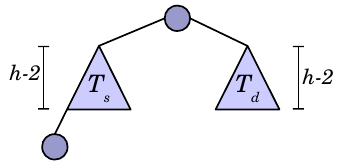
\includegraphics[scale=0.8]{res/Alberobinarioquasicompleto}
\caption{}\label{fig:alberoquasicompleto}
\end{figure}

Allora:
\begin{align*}
	\#_{nodi}(T) = 1+1+\#_{nodi}(T_{s})+\#_{nodi}(T_{d})
\end{align*}
dove:
\begin{align*}
\#_{nodi}(T_{s}) = \#_{nodi}(T_{d})=2^{h-1}-1
\end{align*}
Quindi:
\begin{align*}
\#_{nodi}(T) &= 2+(2^{h-1}-1)+(2^{h-1}-1)\\
&=2 \cdot 2^{h-1} \\
&= 2^{h}
\end{align*}

\end{proof}

\begin{propbox}
L'altezza di un albero binario completo $T$ con $n$ nodi è $h = \lfloor \log n \rfloor$.
\end{propbox}

\begin{proof}
Per la proposizione precedente abbiamo che $2^{h}\leq n \leq 2^{h+1}-1 < 2^{h+1}$, cioè, applicando i logaritmi, $h \leq \log n < h+1$ e quindi, applicando la funzione pavimento, $h \leq \lfloor \log n \rfloor<h+1$.Possiamo concludere che $h=\lfloor \log n \rfloor$.
\end{proof}

\subsection{Operazioni di visita in un albero binario}

\textbf{Visitare} un albero significa esaminare sequenzialmente tutti i suoi nodi. Le tipologie di visita si suddividono in due categorie: le \textbf{visite in profondità} e le \textbf{visite in ampiezza}.

\subsubsection{Visite in profondità}
Esistono tre tipi principali di visite in profondità:
\begin{enumerate}
	\item Nella \textbf{visita in ordine} si visita il sottoalbero sinistro, quindi si esamina la radice e infine si visita il sottoalbero destro;
	\begin{lstlisting}[language=asd,caption={Visita-InOrder(T)}]
	if T != nil then
		Visita-InOrder(T@\rightarrow@left)
		Visita(T)
		Visita-InOrder(T@\rightarrow@right)
	\end{lstlisting}
	\item Nella \textbf{visita in pre-ordine} si visita ricorsivamente prima la radice e quindi si visitano il sottoalbero sinistro e quello destro;
	\begin{lstlisting}[language=asd,caption={Visita-PreOrder(T)}]
	if T != nil then
		Visita(T)
		Visita-PreOrder(T@\rightarrow@left)
		Visita-PreOrder(T@\rightarrow@right)
	\end{lstlisting}

	\item Nella \textbf{visita in post-ordine} si visita ricorsivamente prima il sottoalbero sinistro, poi quello destro ed infine il nodo in radice.
	\begin{lstlisting}[language=asd,caption={Visita-PostOrder(T)}]
	if T != nil then
		Visita-PostOrder(T@\rightarrow@left)
		Visita-PostOrder(T@\rightarrow@right)
		Visita(T)
	\end{lstlisting}
\end{enumerate}

\begin{example}
	Dato l'albero binario:
	\begin{center}
		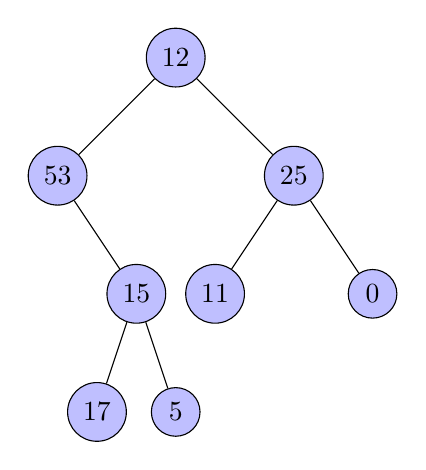
\begin{tikzpicture}
			[level 1/.style={sibling distance=3cm},
			level 2/.style={sibling distance=2cm},
			level 3/.style={sibling distance=1cm},
			every node/.style = {shape=circle, draw, align=center, fill=blue!25!white}]
			\node{12}
			child{
				node{53}
				child[missing]
				child{
					node{15}
					child{
						node{17}
					}
					child{
						node{5}
					}
				}
			}
			child{
				node{25}
				child{
					node{11}
				}
				child{
					node{0}
				}
			};
		\end{tikzpicture}
	\end{center}
	Supponiamo di avere un'operazione di visita che si occuperà di stampare la chiave conservata nel nodo correntemente visitato. Si avrà allora, per ciascuna tipologia di visita, il seguente output:
	\begin{enumerate}
		\item \textbf{Visita in PreOrder:} \texttt{12 53 15 17 5 25 11 0}
		\item \textbf{Visita in InOrder:} \texttt{53 17 15 5 12 11 25 0}
		\item \textbf{Visita in PostOrder:} \texttt{17 5 15 53 11 0 25 12}
	\end{enumerate}
\end{example}

\subsubsection{Visita in ampiezza}
Vediamo ora un altro tipo di visita chiamata \textbf{visita in ampiezza} (o \textbf{per livelli}).

L'idea della visita in ampiezza è quella di visitare dapprima la radice dell'albero, poi i figli della radice, poi i figli dei figli della radice e così via fino alle foglie.

In questo modo i nodi al livello $i$ saranno visitati solo dopo che tutti i nodi del livello $i-1$ sono stati visitati. La difficoltà che si incontra in questo tipo di visita è dato dal fatto che non esiste alcun collegamento tra i nodi di uno stesso livello.

Per questo motivo sarà necessario avvalersi di una \textit{struttura dati ausiliaria} dove inserire le informazioni sull'ordine dei nodi da visitare.

La struttura dati più adatta a questo scopo è la \textbf{coda}. Infatti, ogni volta che si visita un nodo, i suoi figli vengono inseriti in coda. In questo modo, quando si visita un nodo, si è sicuri che tutti i nodi di livello inferiore sono già stati visitati. L'algoritmo~\ref{lst:bfs_tree} mostra come implementare la visita in ampiezza.


\begin{example}
	Si consideri l'albero binario mostrato in Figura~\ref{fig:binary_Tree}. L'algoritmo di visita in ampiezza inizia visitando il nodo in radice che viene inserito in coda:

	\smallskip
	\begin{tblr}{hlines,vlines}
		1 \\
	\end{tblr}
	\smallskip

	La lettura avviene rimuovendo dalla coda l'elemento in testa, quindi il nodo in radice viene rimosso dalla coda e i suoi figli vengono inseriti in coda:
	\smallskip

	\begin{tblr}{hlines,vlines}
		3 & 2 \\
	\end{tblr}
	\smallskip

	Successivamente, il nodo 2 viene rimosso e si inseriscono in coda i suoi nodi figli:
	\smallskip

	\begin{tblr}{hlines,vlines}
		5 & 4 & 3 \\
	\end{tblr}
	\smallskip

	Una volta aver estratto il nodo 3 ed aver inserito i nodi figli, bisogna solo estrarre gli elementi in coda:
	\smallskip

	\begin{tblr}{hlines,vlines}
		7 & 6 & 5 & 4 \\
	\end{tblr}
	\smallskip

	In questo modo la lettura dell'albero in ampiezza produce il seguente output: \texttt{1 2 3 4 5 6 7}
	\begin{center}
		\begin{forest}
			for tree={
				circle,
				draw,
				minimum size=0.7cm,
				fill=blue!25!white,
			}
			[1
			[2
			[4]
			[5]
			]
			[3
			[6]
			[7]
			]
			]
		\end{forest}
		\captionof{figure}{}\label{fig:binary_Tree}
	\end{center}

\end{example}


\begin{lstlisting}[language=asd,label=lst:bfs_tree,caption={BFS(T)}]
// Accodiamo la testa dell'albero
Q = {T}
while Q @\neq@ {} do
	// Leggo la testa della coda
	x = Head(Q)
	Visita(x)
	// Accodo i figli sinistro e destro
	Q = Enqueue(Q, x@\rightarrow@ left)
	Q = Enqueue(Q, x@\rightarrow@ right)
	// Decodo
	Q = Dequeue(Q)
\end{lstlisting}

\section{Alberi binari di ricerca}
Finora abbiamo esplorato le proprietà algebriche delle strutture dati, ma ora ci concentreremo su un tipo particolare di struttura: gli Alberi Binari di Ricerca (ABR). Prima di addentrarci in questo argomento, vale la pena fare un confronto con le strutture dati lineari che abbiamo precedentemente studiato.

Le strutture dati lineari, come le liste, gli array e le code, organizzano i dati in una sequenza unidimensionale, simile a una fila di oggetti allineati in una vetrina. Queste strutture sono efficaci per molte applicazioni, ma possono avere limitazioni quando si tratta di ricerche efficienti o di mantenere un ordine specifico dei dati.

Gli \textbf{alberi binari di ricerca}, al contrario, sfruttando la proprietà \ref{prop:abr} offre vantaggi distinti, in particolare nella ricerca rapida e nell'ordinamento automatico dei dati come si vedrà nei paragrafi successivi.


\begin{axiombox}{Proprietà di ordinamento degli alberi binari di ricerca}\label{prop:abr}
Sia $x$ un nodo in un albero \textsc{ABR}. Se $y$ è un nodo nel sottoalbero sinistro di $x$, allora $y.key \leq x.key$. Se $y$ è un nodo nel sottoalbero destro di $x$, allora $y.key \geq x.key$. In altre parole, i valori più piccoli sono sempre a sinistra e i valori più grandi sono sempre a destra.
\end{axiombox}


\begin{example}
	Si osservi l'albero binario di ricerca in Figura~\ref{fig:binary_search_tree}. In questo albero, per ogni nodo $x$, le chiavi di tutti i nodi nel sottoalbero sinistro di $x$ sono minori o uguali a $x.key$, e le chiavi di tutti i nodi nel sottoalbero destro di $x$ sono maggiori o uguali a $x.key$.

\begin{center}
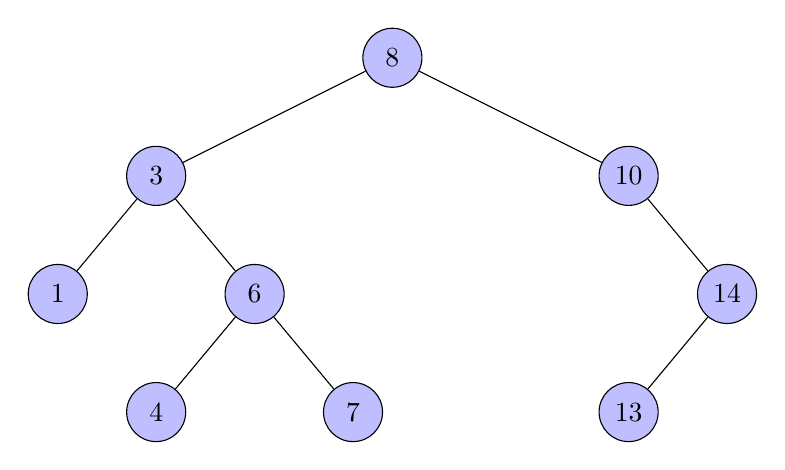
\begin{tikzpicture}
[every node/.style={draw,circle,minimum size=.75cm,fill=blue!25!white},
level 1/.style={sibling distance=6cm},
level 2/.style={sibling distance=2.5cm},
level 3/.style={sibling distance=2.5cm}]
\node{8}
child{
node{3}
child{
  node{1}
}
child{
  node{6}
  child{
    node{4}
  }
  child{
    node{7}
  }
}
}
child{
node{10}
child[missing]
child{
  node{14}
  child{
    node{13}
  }
  child[missing]
}
};
\end{tikzpicture}
\captionof{figure}{Esempio di albero binario di ricerca}\label{fig:binary_search_tree}
\end{center}
\end{example}

Dalla proprietà degli alberi \textsc{ABR} si può dedurre che per ogni albero di ricerca T, sia il sottoalbero sinistro che quello destro sono alberi binari di ricerca. È possibile quindi definire induttivamente un albero binario di ricerca:
\begin{displaymath}
T=
\begin{cases}
\varnothing & \mbox{se vuoto}\\
\begin{cases}
  \text{un sottoalbero \textsc{abr} sinistro }T_{1} \land \ \forall y \in T_{1}(y.key \leq root.key)  \\
  \text{un sottoalbero \textsc{abr} destro }T_{2} \land \ \forall y \in T_{2} (y.key \geq root.key)
\end{cases}
& \mbox{altrimenti}
\end{cases}
\end{displaymath}

\subsection{Operazioni di ricerca}

\subsubsection{Ricerca di un elemento}
Supponiamo di avere un albero binario di ricerca $T$ e si voglia implementare un algoritmo \textsc{Search} che verifichi se un elemento $k$ appartiene all'albero. Sfruttando la proprietà dell'albero \textsc{abr} basterà effettuare un controllo tra $k$ e la chiave memorizzata nel nodo in radice.
\begin{itemize}
\item Se $x.key=k$ abbiamo trovato l'elemento;
\item Se $k < x.key$ allora bisogna cercare
$k$ nel sottoalbero sinistro;
\item Se $k > x.key$ allora bisogna cercare $k$ nel sottoalbero destro.
\end{itemize}
Si ottiene quindi l'algoritmo~\ref{lst:search} molto simile alla ricerca binaria all'interno di un array ordinato. La differenza è che, mentre la ricerca binaria divide l'array in due parti uguali, la ricerca in un albero binario di ricerca divide l'albero in due sottoalberi che possono avere dimensioni molto diverse. Il numero massimo di confronti nel caso peggiore sarà infatti pari alla lunghezza del percorso più lungo, quindi il tempo di esecuzione sarà pari all'altezza dell'albero.

\begin{lstlisting}[language=asd,caption={Search(T,k)},label=lst:search]
if T @\neq@ NIL then
	if T@\rightarrow@key < k then
  		return Search(T@\rightarrow@right, k)
	else if T@\rightarrow@key > k then
  		return Search(T@\rightarrow@left, k)
	else
  		return T
\end{lstlisting}

\subsubsection{Ricerca del minimo e del massimo}
La ricerca del minimo e del massimo sono operazioni banali in un albero binario di ricerca grazie al vincolo di ordinamento globale che questi offrono. Infatti il minimo e il massimo si troveranno sempre nel \textit{nodo più a sinistra e nel nodo più a destra}, rispettivamente.

Ne consegue che il costo della ricerca sarà \textbf{lineare sull'altezza dell'albero} dato che sarà necessario seguire un percorso dalla radice fino a una foglia.

Più precisamente, il minimo si troverà sempre lungo il ramo più a sinistra dell'albero e sarà caratterizzato dal fatto di non avere un figlio sinistro. Dualmente, il massimo sarà il primo nodo del percorso estremo destro che non ha un figlio destro.

\begin{center}
\begin{minipage}{.45\textwidth}

\begin{lstlisting}[language=asd,caption={Search-Min(T)},label=lst:search_min]
	ret = T
	if T @\neq@ NIL then
		x = Search-Min(T@\rightarrow@left)
	if x @\neq@ NIL then
		ret = x
	return ret
\end{lstlisting}
\end{minipage}
\begin{minipage}{.45\textwidth}
	\begin{lstlisting}[language=asd,caption={Search-Max(T)},label=lst:search_max]
	ret = T
	if T @\neq@ NIL then
		x = Search-Max(T@\rightarrow@right)
	if x @\neq@ NIL then
		ret = x
	return ret
\end{lstlisting}
\end{minipage}
\end{center}

\subsubsection{Ricerca del successore e del predecessore}
Dato un nodo in un albero binario di ricerca, a volte è importante trovare il suo successore nell'ordine stabilito da un attraversamento simmetrico. Se tutte le chiavi sono distinte, il successore di un nodo $x$ è il nodo con la chiave più piccola che è maggiore di $x.key$.

La struttura di un albero binario di ricerca consente di determinare il successore di un nodo senza mai dover confrontare le chiavi.

L'algoritmo \textsc{Search-Succ}$(T,k)$ verifica se l'albero $T$ è vuoto, altrimenti si aprono tre strade:
\begin{itemize}
	\item $x.key < k$: la radice contiene un valore minore della chiave, quindi se il successore esiste sarà a destra del nodo $x$, ovvero proprio il risultato che darà la chiamata \textsc{Search-Succ}$(T \rightarrow right, k)$;
	\item $x.key > k$: il successore sarà il risultato della chiamata \textsc{Search-Succ}$(T \rightarrow left,k)$, se $T\rightarrow left = \varnothing$ allora il successore sarà proprio il nodo $x$ (a destra avrò solo valori maggiori di $x$ quindi già so che il miglior candidato è $x$ stesso).
	\item $x.key = k$: è evidente che collassa al caso $x.key<k$, poiché se il successore esiste sarà nel sottoalbero destro.
\end{itemize}

\begin{lstlisting}[language=asd,caption={Search-Succ(T,k)},label=lst:search_succ]
	if T @\neq@ NIL then
		if T@\rightarrow@key @\leq@ k then
			return Search-Succ(T@\rightarrow@right, k)
		else
			x = Search-Succ(T@\rightarrow@left, k)
		if x = NIL then
			return T
		else
			return x
\end{lstlisting}

\subsection{Operazioni di modifica}

\subsubsection{Inserimento di un elemento}
Supponiamo di voler inserire un nodo $x$ di chiave $k$ in un albero $T$. L'operazione di inserimento consiste nell'ottenere un nuovo albero, detto $T'$, posto in questo modo:
\begin{displaymath}
T'= T \cup \{x\}
\end{displaymath}
Supposto che non debbano esserci chiavi duplicate, esistono due casi possibili:
\begin{enumerate}
\item \textbf{L'albero iniziale è vuoto}, quindi basta effettuare un inserimento in testa
\item \textbf{L'albero iniziale non è vuoto}, quindi $x$ deve essere inserito nel sottoalbero vuoto corretto. Infatti, se $x \notin T$, allora inserirlo in $T$ significa cercare un sottoalbero vuoto (o alla peggio una foglia) che soddisfa la proprietà dell'ordinamento.
\end{enumerate}

\begin{lstlisting}[language=asd,caption={Insert(T,k)},label=lst:insert_bst]
if T = NIL then
	x = Alloca()
	x@\rightarrow@key = k
	x@\rightarrow@left = x@\rightarrow@right = NIL
	T = x
else if T@\rightarrow@key < k then
	Insert(T@\rightarrow@right, k)
else
	Insert(T@\rightarrow@left, k)
\end{lstlisting}

\begin{example}
Consideriamo l'albero \ref{fig:binary_search_tree} e supponiamo di voler inserire il nodo 5. L'algoritmo \ref{lst:insert_bst} controlla innanzitutto che l'albero non sia vuoto, successivamente confronta il dato 5 con le varie radici per capire in quale sottoalbero deve richiamarsi. Una volta arrivato al nodo 4, l'algoritmo arriva al caso base ed effettua l'inserimento di un nuovo nodo.
\begin{center}
		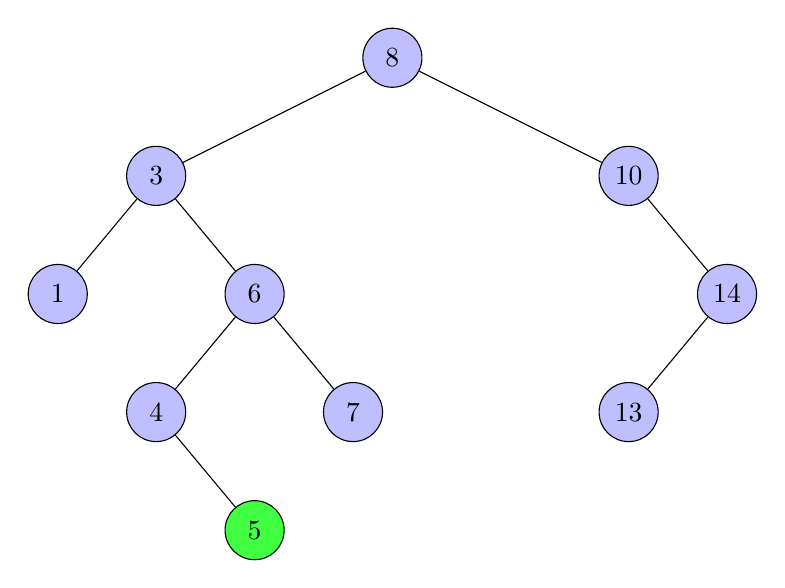
\begin{tikzpicture}
			[every node/.style={draw,circle,minimum size=.75cm,fill=blue!25!white},
			level 1/.style={sibling distance=6cm},
			level 2/.style={sibling distance=2.5cm},
			level 3/.style={sibling distance=2.5cm}]
			\node{8}
			child{
				node{3}
				child{
					node{1}
				}
				child{
					node{6}
					child{
						node{4}
						child[missing]
						child{
							node[fill=green!75!white]{5}
						}
					}
					child{
						node{7}
					}
				}
			}
			child{
				node{10}
				child[missing]
				child{
					node{14}
					child{
						node{13}
					}
					child[missing]
				}
			};
		\end{tikzpicture}
	\captionof{figure}{Esempio di inserimento in un albero binario di ricerca}
\end{center}
\end{example}

\subsubsection{Cancellazione di un nodo}\label{sez:abr_delete}
\paragraph{Eliminiazione di una foglia}
Consideriamo l'albero binario di ricerca mostrato in Figura~\ref{fig:delete-abr-1}. Supponiamo di voler cancellare il nodo con chiave 5. In questo caso il nodo da eliminare non ha figli e possiamo cancellarlo semplicemente impostando il puntatore \texttt{right} del padre a \textsc{nil}. Questo è il caso più semplice di \hypertarget{abr:delete}{cancellazione}.

\begin{center}
\begin{minipage}{.45\textwidth}
\centering
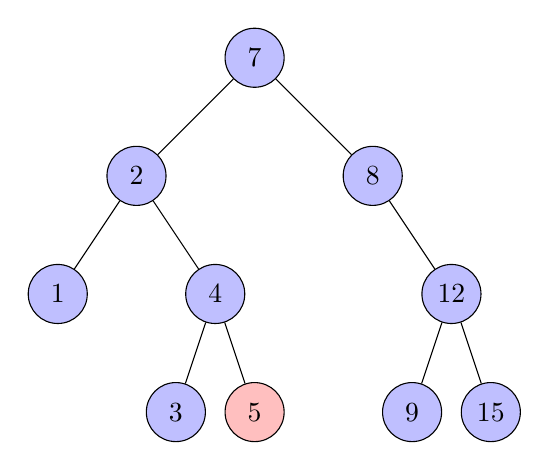
\begin{tikzpicture}
[every node/.style={draw,circle,minimum size=.75cm,fill=blue!25!white},
level 1/.style={sibling distance=3cm},
level 2/.style={sibling distance=2cm},
level 3/.style={sibling distance=1cm}]
\node{7}
child{
node{2}
child{
node{1}
}
child{
node{4}
child{
  node{3}
}
child{
  node[fill=red!25!white]{5}
}
}
}
child{
node{8}
child[missing]
child{
  node{12}
  child{
    node{9}
  }
  child{
    node{15}
  }
}
};
\end{tikzpicture}
\captionof{figure}{Cancellazione in un albero binario di ricerca: caso 1}\label{fig:delete-abr-1}
\end{minipage}
\hfil
\begin{minipage}{.45\textwidth}
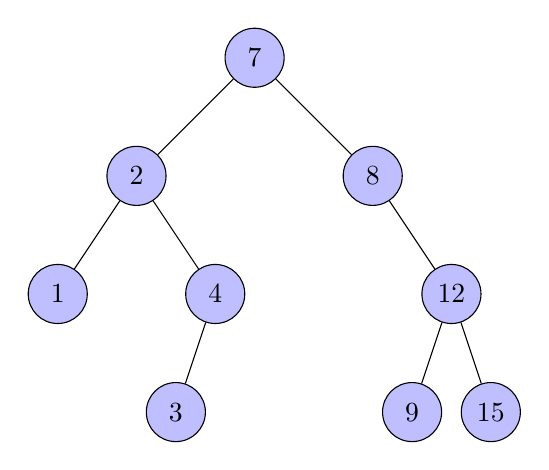
\begin{tikzpicture}
[every node/.style={draw,circle,minimum size=.75cm,fill=blue!25!white},
level 1/.style={sibling distance=3cm},
level 2/.style={sibling distance=2cm},
level 3/.style={sibling distance=1cm}]
\node{7}
child{
node{2}
child{
node{1}
}
child{
node{4}
child{
  node{3}
}
child[missing]
}
}
child{
node{8}
child[missing]
child{
  node{12}
  child{
    node{9}
  }
  child{
    node{15}
  }
}
};
\end{tikzpicture}
\captionof{figure}{Albero risultante dalla cancellazione}\label{fig:delete-abr-1-result}
\end{minipage}
\end{center}
\paragraph{Eliminazione di un nodo con un solo figlio}
Consideriamo ora il caso in cui il nodo da eliminare abbia un solo figlio come nel caso del nodo con chiave 4 mostrato in Figura~\ref{fig:delete-abr-2}. In questa situazione si procede eliminando il nodo e collegando il padre del nodo da eliminare con il figlio del nodo da eliminare. Nel caso in cui il nodo da eliminare sia la radice, allora il figlio del nodo da eliminare diventa la nuova radice dell'albero. (Figura~\ref{fig:delete-abr-2-result})

\begin{center}
\begin{minipage}{.45\textwidth}
\centering

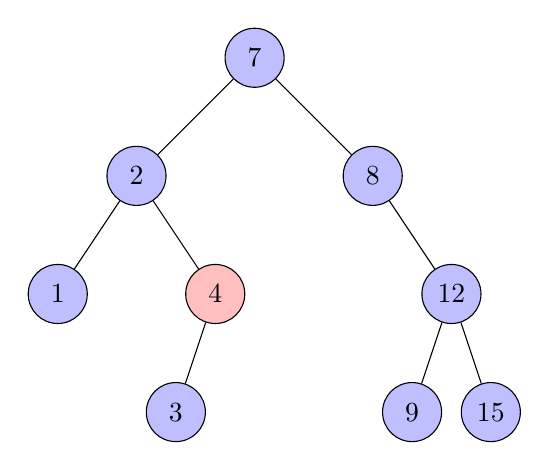
\begin{tikzpicture}
[every node/.style={draw,circle,minimum size=.75cm,fill=blue!25!white},
level 1/.style={sibling distance=3cm},
level 2/.style={sibling distance=2cm},
level 3/.style={sibling distance=1cm}]
\node{7}
child{
node{2}
child{
node{1}
}
child{
node[fill=red!25!white]{4}
child{
  node{3}
}
child[missing]
}
}
child{
node{8}
child[missing]
child{
  node{12}
  child{
    node{9}
  }
  child{
    node{15}
  }
}
};
\end{tikzpicture}
\captionof{figure}{Cancellazione in un albero binario di ricerca: caso 2}\label{fig:delete-abr-2}
\end{minipage}
\begin{minipage}{.45\textwidth}
\centering
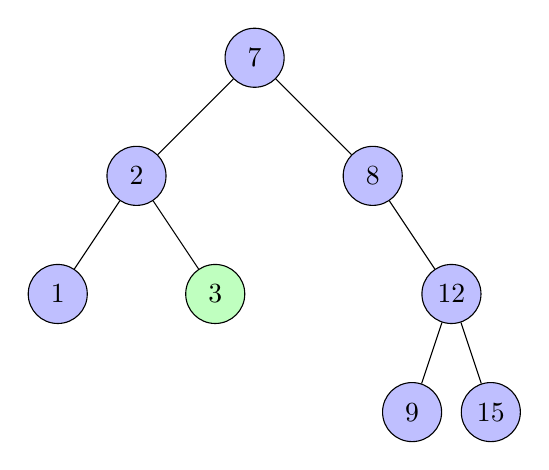
\begin{tikzpicture}
[every node/.style={draw,circle,minimum size=.75cm,fill=blue!25!white},
level 1/.style={sibling distance=3cm},
level 2/.style={sibling distance=2cm},
level 3/.style={sibling distance=1cm}]
	\node{7}
	child{
		node{2}
		child{
			node{1}
		}
		child{
			node[fill=green!25!white]{3}
		}
	}
	child{
		node{8}
		child[missing]
		child{
			node{12}
			child{
				node{9}
			}
			child{
				node{15}
			}
		}
	};
\end{tikzpicture}
\captionof{figure}{Albero risultante dalla cancellazione}\label{fig:delete-abr-2-result}
\end{minipage}
\end{center}
\paragraph{Eliminazione di un nodo con due figli}
Il caso più complesso è quello in cui il nodo da eliminare ha due figli. Per esempio, consideriamo la cancellazione del nodo con chiave 2 all'interno del albero binario di ricerca mostrato in Figura~\ref{fig:delete-abr-3}. In questo caso è necessario trovare il \textbf{successore del nodo da eliminare}, ovvero il nodo con la chiave più piccola nel sottoalbero destro del nodo da eliminare che nel nostro caso è rappresentato dal nodo di chiave 3 (Figura~\ref{fig:delete-abr-3-min}).

Il successore è garantito essere privo di figlio sinistro\footnote{Se così non fosse allora esisterebbe un nodo con chiave minore}, quindi può essere eliminato usando uno dei due casi precedenti. La ricerca del successore si ricondurrà quindi alla ricerca del nodo minimo all'interno del sottoalbero destro del nodo da eliminare. Una volta trovato questo minimo sarà sufficiente \textbf{staccarlo} (Figura \ref{fig:delete-abr-3-min-detach}) dalla sua posizione attuale e sostituirlo al nodo da eliminare. Gli eventuali figli destri del successore verranno poi attaccati al padre. (Figura~\ref{fig:delete-abr-3-result})

Per questo motivo sarà necessario definire tre algoritmi: \textsc{Cancella}$(T,k)$, \textsc{Cancella-Radice}$(T)$ e \textsc{Stacca-Minimo}$(T)$. L'algoritmo \textsc{Cancella}$(T,k)$ è l'algoritmo principale che si occupa di cancellare un nodo $k$ dall'albero $T$. Sulla base dei confronti si determina il percorso da seguire fino a quando non si arriva al nodo da eliminare, sarà poi compito dell'algoritmo \textsc{Delete-Root}$(T)$ di discriminare i casi appena descritti.

\begin{lstlisting}[language=asd,caption={\textsc{Cancella}(T,k)},label=lst:delete]
if T @\neq@ NIL then
	if T@\rightarrow@key < k then
		T@\rightarrow@left = Cancella(T@\rightarrow@left, k)					//Cancellazione nel sottoalbero sx
	else if T@\rightarrow@key > k then
		T@\rightarrow@right = Cancella(T@\rightarrow@right, k)			//Cancellazione nel sottoalbero dx
	else
		T = Delete-Root(T)				    //Cancellazione in radice
return T
\end{lstlisting}

Nel caso in cui $T$ abbia un solo figlio basterà aggiornare $T$ con l'indirizzo del figlio e deallocare la vecchia radice.  Qualora invece il nodo in radice avesse due figli sarà l'algoritmo \textsc{Stacca-Minimo}$(T,P)$ ad occuparsi di staccare il minimo del sottoalbero destro del nodo da eliminare. Il parametro $P$ serve per ricordarsi il padre di $T$ durante la discesa.

\begin{lstlisting}[language=asd,caption={\textsc{Delete-Root}(T)},label=lst:delete-root]
if T @\neq@NIL then
// Caso 1: T ha due figli
if T@$\rightarrow$@ left  @$\neq$@ NIL && T@$\rightarrow$@ right  @$\neq$@ NIL then
 	tmp = Stacca-Minimo(T@$\rightarrow$@ right,T)
 	T @$\rightarrow$@ key = tmp
else
// Caso 2: T ha un solo figlio
 	tmp = T
 	if T@$\rightarrow$@ right @$\neq$@ NIL then
 		T = T @$\rightarrow$@  right
 	else
 		T = T@$\rightarrow$@ left
 	Dealloca(tmp)
return T
\end{lstlisting}

\marker{yellow!50}{yellow!20!black}{\textsc{Stacca-Minimo} non fa altro che restituire la chiave del nodo minimo presente nel sottoalbero sinistro in modo tale da eseguire una sovrascrittura delle chiavi. Dopo di che, aggiorna i puntatori del nodo padre in modo tale che questo venga allacciato ai nodi restanti del sottoalbero destro.}

\begin{lstlisting}[language=asd,caption={\textsc{Stacca-Minimo}(T,P)},label=lst:delete-min]
if T@\neq@NIL then
	//Caso base: T ha un figlio sinistro
	if T@\rightarrow@left @\neq@ NIL then
		return Stacca-Minimo(T@\rightarrow@left, T)
	else
		tmp = T@$\rightarrow$@ key
		// Aggiorno i puntatori del padre
		// Caso 1: T era figlio sinistro del padre
		if P @\rightarrow@left = T then
		  P@\rightarrow@left = T@\rightarrow@right
		// Caso 2: T era figlio destro del padre
		else
		  P@\rightarrow@right = T@\rightarrow@right
		return tmp
\end{lstlisting}

\begin{center}
\begin{minipage}{.45\textwidth}
\centering
	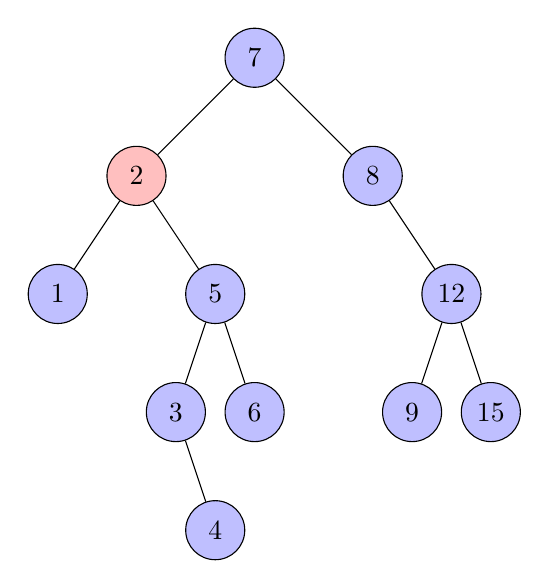
\begin{tikzpicture}
		[every node/.style={draw,circle,minimum size=.75cm,fill=blue!25!white},
		level 1/.style={sibling distance=3cm},
		level 2/.style={sibling distance=2cm},
		level 3/.style={sibling distance=1cm}]
		\node{7}
		child{
			node[fill=red!25!white]{2}
			child{
				node{1}
			}
			child{
				node{5}
				child{
					node{3}
					child[missing]
					child{
						node{4}
					}
				}
				child{
					node{6}
				}
			}
		}
		child{
			node{8}
			child[missing]
			child{
				node{12}
				child{
					node{9}
				}
				child{
					node{15}
				}
			}
		};
	\end{tikzpicture}
	\captionof{figure}{Cancellazione in un albero binario di ricerca: caso 3}\label{fig:delete-abr-3}
\end{minipage}
\begin{minipage}{.45\textwidth}
	\centering
	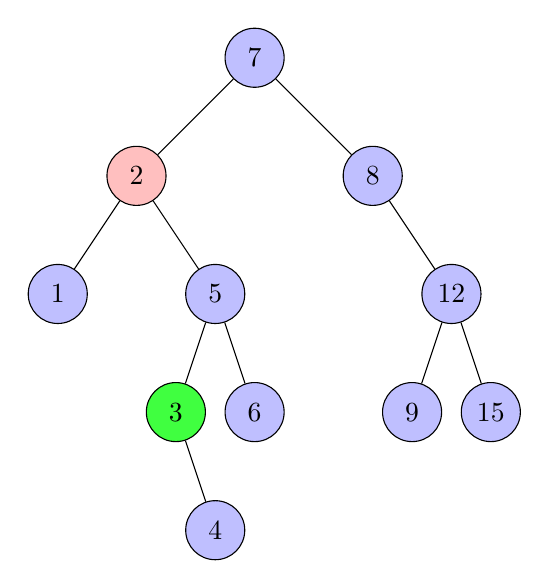
\begin{tikzpicture}
		[every node/.style={draw,circle,minimum size=.75cm,fill=blue!25!white},
		level 1/.style={sibling distance=3cm},
		level 2/.style={sibling distance=2cm},
		level 3/.style={sibling distance=1cm}]
		\node{7}
		child{
			node[fill=red!25!white]{2}
			child{
				node{1}
			}
			child{
				node{5}
				child{
					node[fill=green!75!white]{3}
					child[missing]
					child{
						node{4}
					}
				}
				child{
					node{6}
				}
			}
		}
		child{
			node{8}
			child[missing]
			child{
				node{12}
				child{
					node{9}
				}
				child{
					node{15}
				}
			}
		};
	\end{tikzpicture}
	\captionof{figure}{Individuazione del successore del nodo da eliminare}\label{fig:delete-abr-3-min}
\end{minipage}
\begin{minipage}{.45\textwidth}
\centering
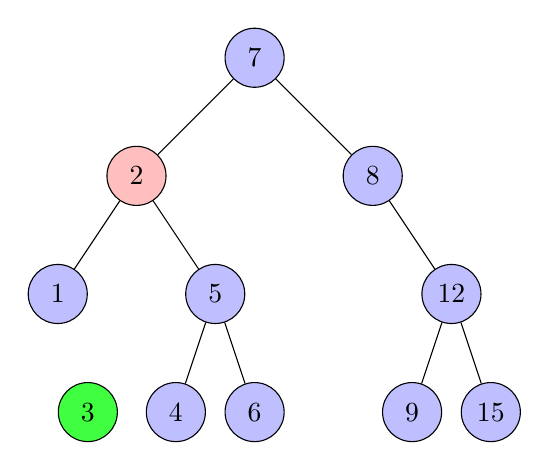
\begin{tikzpicture}
	[every node/.style={draw,circle,minimum size=.75cm,fill=blue!25!white},
	level 1/.style={sibling distance=3cm},
	level 2/.style={sibling distance=2cm},
	level 3/.style={sibling distance=1cm}]
	\node{7}
	child{
		node[fill=red!25!white]{2}
		child{
			node{1}
		}
		child{
			node{5}
			child{
				node[name=4]{4}
			}
			child{
				node{6}
			}
		}
	}
	child{
		node{8}
		child[missing]
		child{
			node{12}
			child{
				node{9}
			}
			child{
				node{15}
			}
		}
	};
	\node[shape=circle, draw, align=center, fill=green!75!white] at ([xshift=-1.5cm]4.east) {3};
\end{tikzpicture}
\captionof{figure}{Staccaggio del successore}\label{fig:delete-abr-3-min-detach}
\end{minipage}
\begin{minipage}{.45\textwidth}
\centering
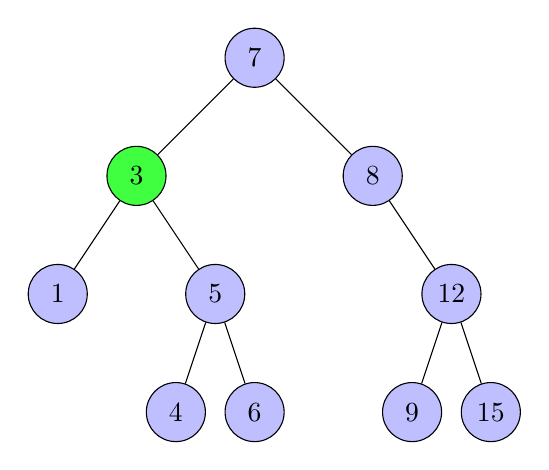
\begin{tikzpicture}
	[every node/.style={draw,circle,minimum size=.75cm,fill=blue!25!white},
	level 1/.style={sibling distance=3cm},
	level 2/.style={sibling distance=2cm},
	level 3/.style={sibling distance=1cm}]
	\node{7}
	child{
		node[fill=green!75!white]{3}
		child{
			node{1}
		}
		child{
			node{5}
			child{
				node{4}
			}
			child{
				node{6}
			}
		}
	}
	child{
		node{8}
		child[missing]
		child{
			node{12}
			child{
				node{9}
			}
			child{
				node{15}
			}
		}
	};
\end{tikzpicture}
\captionof{figure}{Albero risultante dalla cancellazione}\label{fig:delete-abr-3-result}
\end{minipage}
\end{center}

\section{Alberi AVL}
\subsection{Alberi bilanciati}
Gli alberi bilanciati di ricerca sorgono come una soluzione ai problemi di inefficienza che possono emergere negli alberi binari di ricerca. Infatti, la creazione di un albero binario di ricerca non bilanciato, in cui un sottoalbero ha molte più profondità rispetto all'altro, può portare a un'operazione di ricerca con una complessità temporale peggiorativa, che può diventare lineare rispetto al numero di elementi nell'albero. Questo è chiaramente inaccettabile in applicazioni in cui è necessaria una risposta rapida.

Gli \textbf{alberi bilanciati di ricerca} affrontano questo problema stabilendo rigorosi vincoli sulla loro struttura capaci di garantire un buon bilanciamento tra le altezze dei sottoalberi sinistro e destro di ciascun nodo. Questo bilanciamento delle altezze è ottenuto mediante regole di inserimento e rimozione particolari, e il risultato è un albero in cui le operazioni di ricerca, inserimento e cancellazione hanno una complessità temporale tipicamente logaritmica, garantendo prestazioni prevedibili e ottimali in qualsiasi scenario. Nelle prossime sezioni esploreremo le specifiche regole e le varianti di alberi bilanciati di ricerca, come gli alberi AVL e gli alberi rosso-neri per comprendere appieno come questi vincoli migliorino notevolmente l'efficienza delle operazioni sugli alberi binari di ricerca.

\dfn{Alberi bilanciati di ricerca}{
Una classe di alberi binari di ricerca si dice \textbf{bilanciata} se
\begin{displaymath}
	h(T) = \Theta(\log_{2}n) \qquad \mbox{dove } n = |T| \ \mbox{è la cardinalità di T}
\end{displaymath}
}


\begin{osservation}
Gli alberi binari completi appartengono alla classe degli alberi bilanciati.
\end{osservation}

Un'altra classe di alberi binari che soddisfa alle nostre esigenze è quella degli \textbf{alberi perfettamente bilanciati}.

\dfn{Alberi perfettamente bilanciati}{
Un albero binario di ricerca T si dice \textbf{perfettamente bilanciato} (\textbf{APB}) se:
\begin{equation}
	\forall x \in T \qquad ||x \rightarrow left| - |x\rightarrow right||\leq 1
\end{equation}
ovvero la differenza, per ogni nodo di $T$, in valore assoluto tra la cardinalità del sottoalbero sinistro e quello destro è al più uno.
}
\begin{example}
L'albero binario di ricerca in Figura~\ref{fig:perfectly_balanced_tree} è perfettamente bilanciato, infatti per ogni nodo la differenza tra il numero di nodi nel sottoalbero sinistro e destro è al più uno. Preso ad esempio il nodo in radice, la differenza tra i suoi due sottoalberi è:
\begin{displaymath}
| |root \rightarrow left| - |root \rightarrow right||=|2 - 3 | = |-1|=1 \leq 1
\end{displaymath}

Gli alberi perfettamente bilanciati riescono a garantire un tempo di esecuzione logaritmico per le operazioni di ricerca, inserimento e cancellazione. Tuttavia, questa classe di alberi è molto restrittiva, poiché richiede numerosi controlli a fronte di ogni inserimento o cancellazione. Per questo motivo, gli alberi perfettamente bilanciati non sono molto utilizzati in pratica.
\end{example}

\begin{center}
\begin{minipage}{.45\textwidth}
	\centering
	\begin{forest}
	for tree={
		circle,
		draw,
		minimum size=0.5cm,
		fill=blue!25!white,
	}
	[
	[
	[ ]
	[ ]
	]
	[
	[
	[,phantom]
	[]
	]
	[]
	]
	]
\end{forest}
\captionof{figure}{Esempio di albero perfettamente bilanciato}\label{fig:perfectly_balanced_tree}
\end{minipage}
\begin{minipage}{.45\textwidth}
	\centering
	\begin{forest}
		for tree={
			circle,
			draw,
			minimum size=0.5cm,
			fill=blue!25!white,
		}
		[
			[
				[]
				[]
			]
			[]
		]
	\end{forest}
	\captionof{figure}{Esempio di albero non perfettamente bilanciato}\label{fig:not_perfectly_balanced_tree}
\end{minipage}
\end{center}

\subsection{Gli alberi AVL}
La classe di alberi \textbf{AVL (Adelson-Velskii e Landis)} rappresenta una classe di alberi bilanciati con buone prestazioni e gestione relativamente semplice. È praticamente una versione più permissiva di \textsc{APB}.

\dfn{Alberi AVL}{
Un albero $T$ è \textsc{avl} se e solo se:
\begin{equation}\label{avl_prop}
	\forall x \in T \qquad |h(x \rightarrow left) -h(x \rightarrow right)|\leq 1
\end{equation}
ovvero se, per ogni nodo dell'albero, la differenza in modulo dell'altezza del sottoalbero sinistro e il sottoalbero destro è al più uno.
}

Analogamente a quanto visto per le strutture dati precedenti, è possibile definire un albero AVL in modo ricorsivo: un albero binario di ricerca $T$ appartiene alla classe \textsc{AVL} se e soltanto se la differenza tra l'altezza del suo sottoalbero destro e il suo sottoalbero sinistro è minore o uguale di uno e i due sottoalberi appartengono alla classe \textsc{AVL}.

La variabilità negli alberi \textsc{avl} è abbastanza ampia, infatti con lo stesso numero di nodi è possibile generare molti alberi \textsc{avl}. Ma la cosa interessante è che \textbf{ogni albero perfettamente bilanciato è \textsc{avl}} poiché è di fatto un albero completo, il quale rispetta la proprietà di AVL per definizione.

Nel caso degli AVL però non possiamo immediatamente definire una relazione tra l’altezza e il numero dei nodi (con $n$ nodi possiamo infatti generare diversi \textsc{avl} con altezza differente). Per raggiungere il nostro obiettivo dobbiamo restringere la classe \textsc{avl} in una particolare sottoclasse così da far valere la proprietà per tutti gli \textsc{avl}.

Generalmente, una proprietà valida per una sottoclasse non si estende alla superclasse, ma noi andremo a prendere degli alberi AVL con altezza peggiore possibile ed è intuitivo pensare che se per gli alberi peggiori vale $O(\log n)$ allora anche per tutti gli altri la relazione sarà verificata.


\subsection{Alberi \textsc{avl} minimi}
Gli alberi \textsc{avl} minimi sono una sottoclasse degli alberi \textsc{avl} che ci permette di definire una relazione tra l’altezza e il numero dei nodi. Questa classe di alberi è definita come segue:
\dfn{Alberi AVL minimi}{
Fissato $h$, l'\textbf{albero \textsc{avl} minimo} di altezza $h$ è l'albero \textsc{avl} col \textit{minor numero di nodi possibile} sotto il quale l'albero perde la proprietà di essere \textsc{AVL}.
}

\begin{center}
\begin{minipage}{.2\textwidth}
\centering
 \begin{forest}
  for tree={
    circle,
    draw,
    minimum size=0.3cm,
    fill=blue!25!white,
  }
  []
\end{forest}
\end{minipage}
\hfil
\begin{minipage}{.2\textwidth}
\centering
 \begin{forest}
  for tree={
    circle,
    draw,
    minimum size=0.3cm,
    fill=blue!25!white,
  }
  [
    []
    [,phantom]
  ]
\end{forest}
\end{minipage}
\hfil
\begin{minipage}{.3\textwidth}
\centering
 \begin{forest}
  for tree={
    circle,
    draw,
    minimum size=0.3cm,
    fill=blue!25!white,
  }
  [
    [
      []
      [,phantom]
    ]
    []
  ]
\end{forest}
\end{minipage}
\hfil
\begin{minipage}{.3\textwidth}
\centering
 \begin{forest}
  for tree={
    circle,
    draw,
    minimum size=0.3cm,
    fill=blue!25!white,
  }
  [
    [
      [
        []
        [,phantom]
      ]
      []
    ]
    [
    []
    [,phantom]
  ]
  ]
\end{forest}
\end{minipage}
\hfil
\begin{minipage}{.3\textwidth}
\centering
 \begin{forest}
  for tree={
    circle,
    draw,
    minimum size=0.3cm,
    fill=blue!25!white,
  }
  [
    [
    [
      [
        []
        [,phantom]
      ]
      []
    ]
    [
    []
    [,phantom]
  ]
  ]
  [
    [
      []
      [,phantom]
    ]
    []
  ]
  ]
\end{forest}
\end{minipage}
\hfil
\begin{minipage}{.3\textwidth}
\centering
\begin{forest}
    for tree={
      circle,
      draw,
      minimum size=0.3cm,
      fill=blue!25!white,
    }
    [
      [
    [
    [
      [
        []
        [,phantom]
      ]
      []
    ]
    [
    []
    [,phantom]
  ]
  ]
  [
    [
      []
      [,phantom]
    ]
    []
  ]
  ]
  [
    [
      [
        []
        [,phantom]
      ]
      []
    ]
    [
    []
    [,phantom]
  ]
  ]
    ]
  \end{forest}
\end{minipage}
\captionof{figure}{Alberi AVL minimi di altezza 0, 1, 2, 3, 4 e 5}\label{fig:avl_min}
\end{center}

Osservando la Figura~\ref{fig:avl_min} notiamo una certa regolarità: infatti un albero \textsc{AVL} minimo di altezza $h$ sarà sempre composto da due alberi \textsc{AVL} minimi di altezza $h-1$ e $h-2$. Vale infatti la seguente proposizione.


\begin{propbox}
Sia T un albero \textsc{AVL} minimo di altezza $h$, vale quindi la seguente proprietà:
\begin{equation}\label{eq:nodi_avl_minimo}
	N(h) = \left \lbrace \begin{array}{ll}
		h & \mbox{se } h=0,1 \\
		1+ N(h-1) + N(h-2) & \mbox{se } h > 1
	\end{array}
	\right.
\end{equation}
dove $N(h)$ rappresenta il numero di nodi di $T$.

\end{propbox}
\begin{proof}
Procediamo per induzione. Per $h=0$ e $h=1$ è immediato vedere che $N(0)=0$ ed $N(1)=1$, in quanto l'albero vuoto e l'albero con la sola radice sono entrambi alberi \textsc{AVL}.

Per $h>1$, indichiamo con $T_{h}$ l'\textsc{AVL} minimo di altezza $h$. Per definizione, $T_{h}$ avrà almeno un sottoalbero \textsc{AVL} di altezza $h-1$, sia questo il sottoalbero $T_{sx}$. Per assurdo, assumiamo che $T_{sx}$ non sia minimo. Questo vorrà dire che esisterà un albero \textsc{AVL}, detto $T'_{sx}$ di altezza $h-1$ che conterrà il minor numero di nodi per tale altezza. Se consideriamo quindi un albero chiamato $T'_{h}$ costituito dalla radice $r$ e con uno dei sottoalberi proprio l'albero $T'_{sx}$, questo conterrà ovviamente meno nodi dell'albero $T_{h}$.

Questo, però, contraddirebbe l'ipotesi iniziale secondo la quale $T_{h}$ fosse l'\textsc{AVL} minimo di altezza $h$. $T_{h}$ sarà quindi necessariamente costituito da una radice $r$ con sottoalberi gli alberi \textsc{AVL} con numero minimo di nodi $T_{h-1}$ e $T_{h-2}$. Da ciò segue l'equazione~\ref{eq:nodi_avl_minimo}.
\end{proof}


\begin{osservation}
Un albero \textsc{avl} minimo di altezza $h$ con numero di nodi pari ad $n$ è l'albero \textsc{avl} di \textbf{altezza massima} tra tutti gli alberi \textsc{avl} con $n$ nodi. Ciò nonostante questi riescono a mantenere un rapporto logaritmico tra l'altezza e il numero di nodi come si vedrà più avanti.
\end{osservation}


\begin{propbox}
Se $T$ è un albero binario di ricerca appartenente alla classe \textsc{avl} con $n$ nodi e $T'$ è un albero binario di ricerca \textsc{avl} minimo con $n$ nodi allora vale:
\begin{displaymath}
	h(T') \geq h(T)
\end{displaymath}
A parità di nodi, quindi, gli \textsc{avl} minimi sono quelli che hanno l'altezza peggiore.
\end{propbox}
\begin{proof}
Sia $T'$ un \textsc{avl} minimo di altezza $h$ con n nodi. Ciò che vogliamo dimostrare è che, preso un secondo albero \textsc{avl} $T$ con lo stesso numero di nodi di $T'$, si abbia:
\begin{displaymath}
h \leq h'
\end{displaymath}
Per assurdo, supponiamo che $h>h'$. Se esistesse un albero \textsc{avl} T con altezza maggiore di $T'$, si potrebbe ottenere un albero \textsc{avl} minimo $T''$ di altezza $h(T'')=h'$ e con meno nodi di $T'$ contraddicendo così la definizione di \textsc{avl} minimo di $T'$.

Sappiamo, per ipotesi, che l'albero $T$ è più alto di $T'$. È possibile quindi effettuare un taglio da $T$ dei nodi che si trovano ad altezza maggiore di $h'$ ottenendo così un albero $T''$ di altezza $h'$ e con meno nodi di $T'$. Bisogna dimostrare che $T''$ è un albero \textsc{avl}. Per farlo, è sufficiente dimostrare che $T''$ è un albero binario di ricerca e che la differenza tra l'altezza del sottoalbero sinistro e destro di ogni nodo è al più 1.

Supponendo per assurdo che $T''$ non sia \textsc{avl} allora violerebbe la condizione di essere \textsc{avl}: per ogni nodo, cioè, la differenza dei due sottoalberi è al più uno. Supponendo che esista un nodo $x$ che viola la proprietà \textsc{avl} allora i suoi sottoalberi hanno delle altezze maggiori di 1 la cui differenza è maggiore di 1. Se esistesse questo nodo, però, una struttura del genere sarebbe esistita anche nell'albero $T$ in quanto appartenenti all'insieme dei nodi non tagliati. Quindi o $T$ non era un albero \textsc{avl} o $T''$ è sicuramente un albero \textsc{avl}. Quindi $T''$ è un albero \textsc{avl} con la stessa altezza di $T'$ ma con meno nodi. Quindi si ottiene così la contraddizione ricercata.
\end{proof}

\subsection{Relazione tra altezza e numero di nodi}
Sia $n$ il \textbf{numero minimo di nodi} di un albero \textsc{avl} di altezza $h$. È possibile definire una funzione $N(h)$ che restituisce il numero di nodi per un albero \textsc{avl} di altezza $h$.

\begin{table}[h!]
\centering
\begin{tblr}{vlines,hlines,column{1}={primary!80!white}}
	\textbf{h} & 0 & 1 & 2 & 3 & 4 & 5 & 6 & 7 & 8 & 9 & 10 \\
	\textbf{N(h)} & 1 & 2 & 4 & 7 & 12 & 20 & 33 & 54 & 88 & 143 & 232\\
\end{tblr}
\caption{Relazione tra altezza e numero di nodi in un albero \textsc{avl} minimo}
\end{table}

Per qualsiasi albero \textsc{avl} minimo si ha
\begin{displaymath}
N(h) = \left\lbrace
\begin{array}{lc}
	1 & \mbox{se } h=0\\
	2 & \mbox{se } h=1\\
	1 + N(h-1)+N(h-2) & \mbox{se } h \geq 2
\end{array}
\right.
\end{displaymath}
che è molto simile alla funzione di Fibonacci:
\begin{displaymath}
Fib(x) = \left\lbrace
\begin{array}{lc}
	0 & \mbox{se } x=0\\
	1 & \mbox{se } x=1\\
	Fib(x-1)+Fib(x-2) & \mbox{se } x \geq 2
\end{array}
\right.
\end{displaymath}
\begin{table}[h!]
\centering
\begin{tblr}{vlines,hlines,column{1}={primary!80!white}}
	\textbf{h} & 0 & 1 & 2 & 3 & 4 & 5 & 6 & 7 & 8 & 9 & 10 \\
	\textbf{Fib(h)} & 0 & 1 & 1 & 2 & 3 & 5 & 8 & 13 & 21 & 34 & 55 \\
\end{tblr}
\caption{Funzione di Fibonacci}
\end{table}


\begin{propbox}
Si ha:
\begin{equation}\label{nodifib}
	N(h) = Fib(h+3)-1
\end{equation}
\end{propbox}
\begin{proof}
Si dimostra per induzione:
\begin{itemize}
	\item \textbf{Caso base:} Si ha $N(0)=Fib(3)-1=1$ e $N(1)=Fib(4)-1=2$
	\item \textbf{Ipotesi induttiva:} Supponiamo la relazione vera per $h-1$ e $h-2$, ovvero le relazioni:
	\begin{eqnarray*}
		N(h-1) = Fib(h-1+3) = Fib(h+2) \\
		N(h-2) = Fib(h-2+3) = Fib(h+1)
	\end{eqnarray*}
\end{itemize}
Allora:
\begin{eqnarray*}
	N(h) &=& 1+N(h-1)+N(h-2) \\
	&=& 1+ Fib(h+2) -1 + Fib(h+1)-1 \\
	&=& Fib(h+2)+ Fib(h+1)-1 \\
	&=& Fib(h+3)-1
\end{eqnarray*}
\end{proof}

La forma chiusa del numero di Fibonacci è:
\begin{displaymath}
Fib(k) = \frac{1}{\sqrt{5}} \Biggl [ \Bigl(\frac{1+\sqrt{5}}{2}\Bigl)^{h} - \Bigl(\frac{1-\sqrt{5}}{2}\Bigl)^{h} \Biggl]
\end{displaymath}
che, per n sufficientemente grande, può essere approssimato a:
\begin{displaymath}
Fib(h) \cong \frac{1}{\sqrt{5}} \Bigl (\frac{1+\sqrt{5}}{2}\Bigl)^{h}
\end{displaymath}
Quindi:
\begin{displaymath}
\sqrt{5}Fib(h) = \Bigl(\frac{1+\sqrt{5}}{2} \Bigl)^{h} \Longrightarrow h = \log_{\frac{1+\sqrt{5}}{2}}\Bigl(\sqrt{5}Fib(h)\Bigl)
\end{displaymath}
Dunque, applicando l'equazione~\ref{nodifib}:
\begin{displaymath}
N(h)= \frac{1}{\sqrt{5}} \Bigl( \frac{1+ \sqrt{5}}{2}\Bigl)^{h+3} -1
\end{displaymath}

Di conseguenza l'altezza $h$ sarà logaritmica rispetto al numero di nodi. Infatti, indicato con $n$ il numero di nodi di un albero \textsc{AVL} minimo di altezza $h$ si ottiene:
\begin{eqnarray*}
n &=& \frac{1}{\sqrt{5}} \Bigl( \frac{1+ \sqrt{5}}{2}\Bigl)^{h+3} -1 \\
\sqrt{5}(n+1) &=& \Bigl(\frac{1+\sqrt{5}}{2}\Bigl)^{h+3} \\
\Rightarrow  h+3 &=& \log_{\frac{1+\sqrt{5}}{2}} (\sqrt{5}(n+1)) \\
\Rightarrow  h &=& \log_{\frac{1+\sqrt{5}}{2}}(\sqrt{5}(n+1))-3 \\
&=& \frac{\log_{2}(\sqrt{5}(n+1))}{\log_{2}\bigl(\frac{1+\sqrt{5}}{2}\bigl)}-3 \\
&=& \Theta(\log n)
\end{eqnarray*}

\subsection{Implementazione di un albero AVL}

Poiché la definizione di albero \textsc{avl} è legata all'altezza, bisogna trovare un modo per reperire tale informazione per ciascun nodo dell'albero. Per calcolare l'altezza si potrebbe applicare un algoritmo ricorsivo. Infatti, un albero binario o risulta vuoto e la sua altezza sarà $-1$ oppure è composto da una radice dalla quale si radicano eventualmente due alberi binari:
\begin{equation}
h = 1 + max(T\rightarrow left, \; T\rightarrow right)
\end{equation}

Si ottiene in questo modo l'algoritmo~\ref{alg:height} per il calcolo dell'altezza di un albero binario.

\begin{lstlisting}[language=asd,caption={Altezza(T)},label=alg:height]
if T = NIL then
return -1
else
return 1 + max(Altezza(T@\rightarrow@left), Altezza(T@\rightarrow@right))
\end{lstlisting}

L'algoritmo~\ref{alg:height} risulta troppo pesante da utilizzare ogni qualvolta si voglia effettuare un controllo del corretto bilanciamento in un albero \textsc{AVL} in quanto questo risulta lineare sul numero dei nodi dell'albero del quale calcola l'altezza. Per questo motivo può risultare più pratico inserire un nuovo campo, denominato $h$, all'interno di ciascun nodo, in modo tale da ridurre il tempo di ``calcolo'' dell'altezza. Si ottiene quindi un nodo come mostrato in Figura~\ref{fig:nodo_avl}. Il calcolo dell'altezza diventa quindi un semplice accesso in lettura del campo $h$ del nodo. Si ottiene quindi una versione migliore dell'algoritmo \textsc{Altezza}:

\begin{lstlisting}[language=asd,caption={Altezza(T)},label={alg:height_avl}]
if T = NIL then
return -1
else
return T@\rightarrow@h
\end{lstlisting}

\begin{figure}[ht!]
\centering
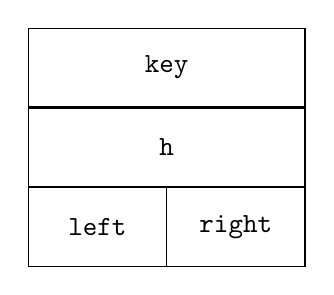
\begin{tikzpicture}[font=\ttfamily,minimum height=1cm]
\node (Key) [rectangle,draw,minimum width=10em] {\texttt{key}};
\node (Height) [rectangle,draw,anchor=north,minimum width=10em] at (Key.south) {\texttt{h}};
\node (LeftChild) [rectangle,draw,anchor=north west,minimum width=5em] at (Height.south west) {\texttt{left}};
\node (RightChild) [rectangle,draw,anchor=north east,minimum width=5em] at (Height.south east) {\texttt{right}};
\end{tikzpicture}
\caption{Nodo di un albero AVL}\label{fig:nodo_avl}
\end{figure}

\subsection{Inserimento in un albero AVL}
Consideriamo un generico albero \textsc{avl} $T$, che sappiamo essere anche binario di ricerca oltre che completo. Applicare l'algoritmo~\ref{lst:insert} per effettuare l'\textbf{inserimento di un nodo} all'interno di $T$ non è sufficiente di per sè per costruire un albero binario di ricerca che soddisfi la proprietà~\ref{avl_prop}. Sarà necessario quindi modificare l'algoritmo introducendo un'algoritmo che effettui un controllo sul bilanciamento e, nel caso si verifichi uno sbilanciamento dell'albero, lo rimetta ``a posto''.

\begin{lstlisting}[language=asd,caption={\textsc{Insert-AVL(T,k)}},label=lst:insert-avl]
if T @\neq@ NIL then
	if T@\rightarrow@ key < k then
		T@\rightarrow@ right = Insert-AVL(T@\rightarrow@ right, k)
		T = Bilancia-Destra(T)
	else if T@\rightarrow@ key > k then
		T@\rightarrow@ left = Insert-AVL(T@\rightarrow@ left, k)
		T = Bilancia-Sinistra(T)
	else
		T = Alloca-Nodo-AVL()
		T@\rightarrow@ key = k
		T@\rightarrow@ left = T@\rightarrow@ right = NIL
		T@\rightarrow@ h = 0
return T
\end{lstlisting}

Per non aggravare il costo computazionale dell'algoritmo \textsc{Insert} (Algoritmo~\ref{lst:insert-avl}) ci aspettiamo che le operazioni all'interno degli algoritmi di bilanciamento abbiano un costo costante $\Theta(1)$. Lo sbilanciamento in un albero \textsc{avl} può essere risolto con una \textbf{sequenza di operazioni di bilanciamento}, anche dette \textbf{rotazioni}, che staranno alla base degli algoritmi \textsc{Bilancia-Sinistra} (Algoritmo~\ref{lst:bilancia-sx}) e \textsc{Bilancia-Destra}.

\subsection{Le rotazioni}
Le rotazioni sono delle operazioni che permettono di ripristinare le proprietà di un albero bilanciato a fronte di operazioni che ne modificano la struttura. Queste sono di due tipi: \textbf{sinistra} e \textbf{destra}\footnote{Per destra e sinistra si intende il sottoalbero che scatena lo sbilanciamento in un nodo e non il senso della rotazione.}. Oltre alle rotazioni singole a sinistra e a destra, è possibile effettuare anche delle \textbf{rotazioni doppie} come la rotazione doppia a sinistra, ovvero una rotazione a sinistra seguita da una rotazione a destra\footnote{La rotazione doppia a destra è duale}.

\subsubsection{La rotazione sinistra}
Consideriamo l'albero mostrato in Figura~\ref{Avl_insert1.png}. Ciascun sottoalbero che si dirama dai nodi $x$ e $y$ hanno altezza $h$ in modo tale che il vertice $x$ non vede alcuno sbilanciamento, vale infatti:
\begin{displaymath}
||x\rightarrow left| - |x \rightarrow right|| = |(h+1) - h| = 1 \leq 1
\end{displaymath}
Effettuando un inserimento di un nodo nel sottoalbero $A$ si ottiene una violazione in radice della proprietà~\ref{avl_prop} (Figura~\ref{Avl_insert2.png}). Infatti, aggiungendo un nodo in $A$, si modifica la sua altezza che, da $h$, diventa $h+1$. Questo inserimento fa scendere l'albero radicato nel nodo $y$ ad una altezza $h+2$. Si ha così la violazione:
\begin{displaymath}
| |x \rightarrow left| - |x \rightarrow right||=|(h+2 )- h |=2 \nleq 1
\end{displaymath}

\begin{center}
\begin{minipage}{.45\textwidth}
\centering
\begin{tikzpicture}
\tikzset{
level 1/.style={sibling distance=2cm},
level 2/.style={sibling distance=1.5cm},
level 3/.style={sibling distance=0.5cm},
itria/.style={isosceles triangle,draw, dashed,shape border rotate=90,isosceles triangle stretches=true, minimum height=10mm,minimum width=12mm,inner sep=0,yshift={-20mm},fill=blue!25!white},
btria/.style={isosceles triangle,draw,dashed,shape border rotate=90,isosceles triangle stretches=true, minimum height=20mm,minimum width=12mm,inner sep=0,yshift={-20mm},fill=red!25!white},
mynode/.style={
  circle,
  draw,
  minimum size=0.5cm,
  fill=blue!25!white
}
}
\node[mynode,name=root]{x}
[child anchor=north]
child
{
  node[mynode,name=root_sx]{y}
    child
    {
     node[itria,name=A_tree]{A}
    }
    child
    {
      node[itria,name=B_tree]{B}
    }
}
child
{
  node[itria,name=C_tree]{C}
};
\node[anchor=east]at(root.west){$+1$};
\node[anchor=east]at(root_sx.west){$+0$};
\end{tikzpicture}
\captionof{figure}{Albero \textsc{AVL} bilanciato: accanto a ciascun vertice è presente la differenza, in valore assoluto, tra le altezze dei sottoalberi.\label{Avl_insert1.png}}
\end{minipage}
\hfil
\begin{minipage}{.45\textwidth}
\centering
\begin{tikzpicture}
\tikzset{
level 1/.style={sibling distance=3cm},
level 2/.style={sibling distance=1.5cm},
level 3/.style={sibling distance=0.75cm},
itria/.style={isosceles triangle,draw, dashed,shape border rotate=90,isosceles triangle stretches=true, minimum height=10mm,minimum width=12mm,inner sep=0,yshift={-20mm},fill=blue!25!white},
btria/.style={isosceles triangle,draw,dashed,shape border rotate=90,isosceles triangle stretches=true, minimum height=20mm,minimum width=12mm,inner sep=0,yshift={-20mm},fill=red!25!white},
mynode/.style={
  circle,
  draw,
  minimum size=0.5cm,
  fill=blue!25!white
}
}
\node[mynode,name=root]{x}
[child anchor=north]
child
{
  node[mynode,name=root_sx]{y}
    child
    {
      node[btria,name=A_tree]{A}
    }
    child
    {
      node[itria,name=B_tree]{B}
    }
}
child
{
 node[itria,name=root_dx]{C}
};
\node[anchor=east]at(root.west){$+2$};
\node[anchor=east]at(root_sx.west){$+1$};
\end{tikzpicture}
\captionof{figure}{Albero \textsc{AVL} sbilanciato: il nodo $x$ vede aumentata la sua altezza\label{Avl_insert2.png}}
\end{minipage}
\end{center}

Come è possibile sistemare la violazione in questa situazione? Essendo stato il sottoalbero sinistro $A$ ad aver generato la violazione nel nodo $x$ si adotterà un'operazione di \textbf{rotazione singola sinistra} che avrà l'effetto di ruotare il nodo $x$ con il suo nodo figlio sinistro, ovvero il nodo $y$. L'operazione è molto semplice e consta dei seguenti passaggi:
\begin{enumerate}
\item Il nodo $y$, ovvero il figlio sinistro del nodo in cui si riscontra la violazione della proprietà~\ref{avl_prop}, \textbf{sale in radice};
\item Il nodo $x$ diventa \textbf{figlio destro} del nodo $y$;
\item Nel momento in cui $y$ ha come figlio destro il nodo $x$ e come figlio sinistro il vecchio albero $A$, si sposta l'albero $B$ come \textbf{figlio sinistro} del nodo $x$. È corretto fare questo spostamento in quanto tutti i nodi di $B$ continuano a stare a destra del nodo $y$ e a sinistra del nodo $x$.
\end{enumerate}

\begin{center}
\begin{minipage}{.45\textwidth}
\centering
\begin{tikzpicture}
\tikzset{
level 1/.style={sibling distance=3cm},
level 2/.style={sibling distance=1.5cm},
level 3/.style={sibling distance=0.75cm},
itria/.style={isosceles triangle,draw, dashed,shape border rotate=90,isosceles triangle stretches=true, minimum height=10mm,minimum width=12mm,inner sep=0,yshift={-20mm},fill=blue!25!white},
btria/.style={isosceles triangle,draw,dashed,shape border rotate=90,isosceles triangle stretches=true, minimum height=20mm,minimum width=12mm,inner sep=0,yshift={-20mm},fill=red!25!white},
mynode/.style={
  circle,
  draw,
  minimum size=0.5cm,
  fill=blue!25!white
}
}
\node[mynode,name=root]{x}
[child anchor=north]
child
{
  node[mynode,name=root_sx]{y}
    child
    {
      node[btria,name=A_tree]{A}
    }
    child[dashed]
    {
      node[itria,name=B_tree]{B}
    }
}
child
{
  node[itria,name=C_tree]{C}
};
\draw[->,red,thick](root_sx.north)to[bend left=35](root.west);
\draw[-,dashed,red,opacity=.8](B_tree)--(root);
\node[anchor=west]at(root.east){$+2$};
\node[anchor=east]at(root_sx.west){$+1$};
\end{tikzpicture}
\captionof{figure}{Rotazione singola sinistra}
\end{minipage}
\hfil
\begin{minipage}{.45\textwidth}
\centering
\begin{tikzpicture}
\tikzset{
level 1/.style={sibling distance=2cm},
level 2/.style={sibling distance=1.5cm},
level 3/.style={sibling distance=0.75cm},
itria/.style={isosceles triangle,draw, dashed,shape border rotate=90,isosceles triangle stretches=true, minimum height=10mm,minimum width=12mm,inner sep=0,yshift={-10mm},fill=blue!25!white},
btria/.style={isosceles triangle,draw,dashed,shape border rotate=90,isosceles triangle stretches=true, minimum height=20mm,minimum width=12mm,inner sep=0,yshift={-20mm},fill=red!25!white},
mynode/.style={
  circle,
  draw,
  minimum size=0.5cm,
  fill=blue!25!white
}
}
\node[mynode,name=root]{y}
[child anchor =north]
child
{
  node[btria,name=A_tree]{A}
}
child{
  node[mynode,name=root_dx]{x}
    child{
      node[itria,name=B_tree]{B}
    }
    child{
    node[itria,name=C_tree]{C}
    }
};
\node[anchor=west]at(root.east){$+0$};
\node[anchor=west]at(root_dx.east){$+0$};
\end{tikzpicture}
\captionof{figure}{Albero risultante dopo la rotazione singola sinistra\label{RotazioneSS_avl.png}}
\end{minipage}
\end{center}

In questo modo l'albero $A$ è salito di un livello mentre l'albero $C$ è sceso di un livello. Si osserva inoltre che, a fronte di un inserimento (che determina una rotazione), \textbf{l'operazione di ribilanciamento ripristina l'altezza dell'albero}. Infatti prima e dopo la rotazione si avrà: \[T \rightarrow h = h+2\] Si ottiene così l'albero in Figura~\ref{RotazioneSS_avl.png} che è ancora un albero \textsc{avl}. Infatti:
\begin{displaymath}
| |x \rightarrow left| - |x \rightarrow right||=|(h+1) - (h+1) |= 0 \leq 1
\end{displaymath}

L'algoritmo \textsc{Rotazione-Sx}(Algoritmo~\ref{lst:rotazione-sx}) prende in ingresso l'indirizzo della testa dell'albero e deve lavorare su due nodi: la radice che viene data in ingresso e la radice del sottoalbero sinistro che genera lo sbilanciamento. È facile vedere che l'algoritmo~\ref{lst:rotazione-sx} è eseguibile a tempo costante.

\begin{lstlisting}[language=asd,caption={Rotazione-Sx(T)},label=lst:rotazione-sx]
newT = T@\rightarrow@left
T@\rightarrow@left = newT@\rightarrow@right
newT@\rightarrow@right = T
T@\rightarrow@h = max(Altezza(T@\rightarrow@left), Altezza(T@\rightarrow@right))+1
newT@\rightarrow@h = max(Altezza(newT@\rightarrow@left), Altezza(newT@\rightarrow@right))+1
return newT
\end{lstlisting}

L'operazione di rotazione singola sinistra non fa altro che sollevare di un livello il sottoalbero $A$ e far scendere $C$. Il sottoalbero $B$ resta allo stesso livello dopo l'operazione di rotazione. Quindi se l'inserimento venisse fatto in $B$ determinando un'incremento dell'altezza di $B$ (sbilanciando di conseguenza il nodo $x$), l'operazione di rotazione singola sinistra lascerebbe immutato lo sbilanciamento.

Per questo motivo sarà necessario utilizzare una doppia operazione di bilanciamento che consiste di una prima rotazione a destra per portarci nel caso di uno sbilanciamento a sinistra e successivamente ripristinare l'albero con una rotazione a sinistra.

\subsubsection{La rotazione destra}
La rotazione destra è duale alla rotazione sinistra. Si consideri l'albero \textsc{avl} mostrato in Figura~\ref{fig:avl-rotazionedx}. In questo caso l'inserimento di un nodo nel sottoalbero $B$ del figlio destro della radice genera una violazione della proprietà~\ref{avl_prop} come si vede in Figura~\ref{fig:avl-sbilanciatodx}. Infatti:
\begin{displaymath}
| |x \rightarrow left| - |x \rightarrow right||=|(h) - (h+2) |=2 \nleq 1
\end{displaymath}

\begin{center}
\begin{minipage}{.45\textwidth}
\centering
\begin{tikzpicture}
\tikzset{
    level 1/.style={sibling distance=2cm},
    level 2/.style={sibling distance=1.5cm},
    level 3/.style={sibling distance=0.5cm},
    itria/.style={isosceles triangle,draw, dashed,shape border rotate=90,isosceles triangle stretches=true, minimum height=10mm,minimum width=12mm,inner sep=0,yshift={-10mm},fill=blue!25!white},
    btria/.style={isosceles triangle,draw,dashed,shape border rotate=90,isosceles triangle stretches=true, minimum height=20mm,minimum width=12mm,inner sep=0,yshift={-20mm},fill=red!25!white},
     mynode/.style={
       	circle,
       	draw,
       	minimum size=0.5cm,
       	fill=blue!25!white
    }
  }
  \node[mynode, name=root]{x}
  [child anchor=north]
  child
  {
      node[itria, name=C_tree]{C}
  }
  child
  {
    node[mynode, name=root_dx]{y}
    child
    {
        node[itria, name=A_tree]{A}
    }
    child
    {
        node[itria, name=B_tree]{B}
    }
  };
\node[anchor=west]at(root.east){$+1$};
\node[anchor=west]at(root_dx.east){$+0$};
\end{tikzpicture}
\captionof{figure}{Albero \textsc{avl} ben bilanciato\label{fig:avl-rotazionedx}}
\end{minipage}
\hfil
\begin{minipage}{.45\textwidth}
\centering
\begin{tikzpicture}
  \tikzset{
    level 1/.style={sibling distance=2cm},
    level 2/.style={sibling distance=1.5cm},
    level 3/.style={sibling distance=0.5cm},
    itria/.style={isosceles triangle,draw, dashed,shape border rotate=90,isosceles triangle stretches=true, minimum height=10mm,minimum width=12mm,inner sep=0,yshift={-10mm},fill=blue!25!white},
    btria/.style={isosceles triangle,draw,dashed,shape border rotate=90,isosceles triangle stretches=true, minimum height=20mm,minimum width=12mm,inner sep=0,yshift={-20mm},fill=red!25!white},
    mynode/.style={
      circle,
      draw,
      minimum size=0.5cm,
      fill=blue!25!white
    }
  }
  \node[mynode, name=root]{x}
  [child anchor= north]
  child
  {
    node[itria, name=C_tree]{C}
  }
  child
  {
    node[mynode, name=root_dx]{y}
    child
    {
        node[itria, name=A_tree]{A}
    }
    child
    {
        node[btria, name=B_tree]{B}
    }
  };
\node[anchor=west]at(root.east){$+2$};
\node[anchor=west]at(root_dx.east){$+1$};
\end{tikzpicture}
\captionof{figure}{Albero \textsc{AVL} sbilanciato\label{fig:avl-sbilanciatodx}}
\end{minipage}
\end{center}

In questo caso si applica una rotazione singola destra che ha l'effetto di far scendere il sottoalbero $C$ e far salire il sottoalbero $B$. L'altezza del sottoalbero $A$ rimane invariata come mostrato in Figura\ref{fig:rotazionedx}.

\begin{center}
\begin{minipage}{.45\textwidth}
\centering
\begin{tikzpicture}
  \tikzset{
    level 1/.style={sibling distance=2cm},
    level 2/.style={sibling distance=1.5cm},
    level 3/.style={sibling distance=0.5cm},
    itria/.style={isosceles triangle,draw, dashed,shape border rotate=90,isosceles triangle stretches=true, minimum height=10mm,minimum width=12mm,inner sep=0,yshift={-10mm},fill=blue!25!white},
    btria/.style={isosceles triangle,draw,dashed,shape border rotate=90,isosceles triangle stretches=true, minimum height=20mm,minimum width=12mm,inner sep=0,yshift={-20mm},fill=red!25!white},
    mynode/.style={ circle,draw, minimum size=0.5cm,fill=blue!25!white}
  }
  \node[mynode, name=root]{x}
  [child anchor = north]
  child
  {
    node[itria, name=C_tree]{C}
  }
  child
  {
    node[mynode, name=root_dx]{y}
    child [dashed]
    {
        node[itria, name=A_tree]{A}
    }
    child
    {
        node[btria, name=B_tree]{B}
    }
};
 \draw[->,red,thick](root_dx)to[bend right=35](root.east);
   \node[anchor=east]at(root.west){$+2$};
 \node[anchor=west]at(root_dx.east){$+1$};
 \draw[dashed,red](A_tree)--(root);
\end{tikzpicture}
\captionof{figure}{Rotazione singola destra\label{fig:rotazionedx}}
\end{minipage}
\hfil
\begin{minipage}{.45\textwidth}
\centering
\begin{tikzpicture}
\tikzset{
    level 1/.style={sibling distance=2cm},
    level 2/.style={sibling distance=1.5cm},
    level 3/.style={sibling distance=0.5cm},
    itria/.style={isosceles triangle,draw, dashed,shape border rotate=90,isosceles triangle stretches=true, minimum height=10mm,minimum width=12mm,inner sep=0,yshift={-10mm},fill=blue!25!white},
    btria/.style={isosceles triangle,draw,dashed,shape border rotate=90,isosceles triangle stretches=true, minimum height=20mm,minimum width=12mm,inner sep=0,yshift={-20mm},fill=red!25!white},
    mynode/.style={
      circle,
      draw,
      minimum size=0.5cm,
      fill=blue!25!white
    },
  }
  \node[mynode, name=root]{y}
  [child anchor = north]
  child
  {
      	node[mynode, name=root_sx]{x}
       child
       {
          	node[itria, name=C_tree]{C}
       }
       child
       {
          	node[itria, name=A_tree]{A}
       }
}
child
{
      	node[btria, name=B_tree]{B}
  };
\node[anchor=east]at(root.west){$+1$};
\node[anchor=west]at(root_sx.east){$+0$};
\end{tikzpicture}
\captionof{figure}{Albero risultante dopo la rotazione singola destra\label{fig:rotazionedx2}}
\end{minipage}
\end{center}

L'algoritmo \textsc{Rotazione-Dx} (Algoritmo~\ref{lst:rotazione-dx}) è duale all'algoritmo \textsc{Rotazione-Sx} (Algoritmo~\ref{lst:rotazione-sx}).

\begin{lstlisting}[language=asd,caption={Rotazione-Dx(T)},label=lst:rotazione-dx]
newT = T@\rightarrow@right
T@\rightarrow@right = newT@\rightarrow@left
newT@\rightarrow@left = T
T@\rightarrow@h = max(Altezza(T@\rightarrow@left), Altezza(T@\rightarrow@right))+1
newT@\rightarrow@h = max(Altezza(newT@\rightarrow@left), Altezza(newT@\rightarrow@right))+1
return newT
\end{lstlisting}
\subsubsection{La doppia rotazione sinistra}
Si consideri l'albero $T$ come mostrato in Figura~\ref{fig:albero-avl-case2}. I sottoalberi $A$ e $D$ hanno altezza $h-2$ mentre i sottoalberi $B$ e $C$ hanno altezza $h-3$. L'albero radicato in $x$ risulta così ben bilanciato, infatti vale:
\begin{displaymath}
||x \rightarrow left| - |x \rightarrow right|| = |(h+1)-(h)| = +1 \leq 1
\end{displaymath}

\begin{center}
\begin{minipage}{.45\textwidth}
\centering
\begin{tikzpicture}
  \tikzset{
    level 1/.style={sibling distance=3cm},
    level 2/.style={sibling distance=2cm},
    level 3/.style={sibling distance=1.5cm},
    itria/.style={isosceles triangle,draw, dashed,shape border rotate=90,isosceles triangle stretches=true, minimum height=10mm,minimum width=12mm,inner sep=0,yshift={-10mm},fill=blue!25!white},
     btria/.style={isosceles triangle,draw,dashed,shape border rotate=90,isosceles triangle stretches=true, minimum height=20mm,minimum width=12mm,inner sep=0,yshift={-20mm},fill=red!25!white},
    ctria/.style={isosceles triangle,draw, dashed,shape border rotate=90,isosceles triangle stretches=true, minimum height=20mm,minimum width=12mm,inner sep=0,yshift={-20mm},fill=blue!25!white},
    mynode/.style={
       	circle,
       	draw,
       	minimum size=0.5cm,
       	fill=blue!25!white
    },
  }
  \node[mynode, name=root]{x}
  [child anchor = north]
  child
  {
    node[mynode,name=root_sx]{y}
    child
    {
      node[ctria, name=A_tree]{A}
    }
    child
    {
      node[mynode,name=y_dx]{z}
      child
      {
        node[itria, name=B_tree]{B}
      }
      child
      {
        node[itria, name=C_tree]{C}
      }
    }
  }
  child
  {
  node[ctria, name=D_tree]{D}
  };
\node[anchor=west]at(y_dx.east){$+0$};
\node[anchor=west]at(root_sx.east){$+0$};
\node[anchor=west]at(root.east){$+1$};
\end{tikzpicture}
\captionof{figure}{Albero \textsc{avl} ben bilanciato\label{fig:albero-avl-case2}}
\end{minipage}
\hfil
\begin{minipage}{.45\textwidth}
\centering
\begin{tikzpicture}
\tikzset{
    level 1/.style={sibling distance=3cm},
    level 2/.style={sibling distance=2cm},
    level 3/.style={sibling distance=1.5cm},
    itria/.style={isosceles triangle,draw, dashed,shape border rotate=90,isosceles triangle stretches=true, minimum height=10mm,minimum width=12mm,inner sep=0,yshift={-10mm},fill=blue!25!white},
     btria/.style={isosceles triangle,draw,dashed,shape border rotate=90,isosceles triangle stretches=true, minimum height=20mm,minimum width=12mm,inner sep=0,yshift={-20mm},fill=red!25!white},
    ctria/.style={isosceles triangle,draw, dashed,shape border rotate=90,isosceles triangle stretches=true, minimum height=20mm,minimum width=12mm,inner sep=0,yshift={-20mm},fill=blue!25!white},
    mynode/.style={
       	circle,
       	draw,
       	minimum size=0.5cm,
       	fill=blue!25!white
    },
  }
  \node[mynode, name=root]{x}
  [child anchor = north]
  child {
    node[mynode,name=root_sx]{y}
    child{
      node[ctria, name=A_tree]{A}
    }
    child{
      node[mynode,name=y_dx]{z}
      child
      {
        node[btria, name=B_tree]{B}
      }
      child
      {
        node[itria, name=C_tree]{C}
      }
    }
  }
  child {
    node[ctria, name=D_tree]{D}
  };
\node[anchor=west]at(y_dx.east){$+1$};
\node[anchor=west]at(root_sx.east){$+1$};
\node[anchor=west,red]at(root.east){$+2$};
\end{tikzpicture}
\captionof{figure}{Inserimento nel sottoalbero $B$\label{fig:sbilanciamento-case2}}
\end{minipage}
\end{center}

Supponiamo di inserire un nodo nel sottoalbero $B$ radicato in $z$. Ovviamente, a seguito dell'inserimento l'altezza di tale sottoalbero risulterà incrementata causando uno sbilanciamento sul nodo $x$ dato dal suo sottoalbero sinistro come mostrato in Figura \ref{fig:sbilanciamento-case2}:
\begin{displaymath}
||x \rightarrow left| - |x \rightarrow right|| = |(h)-(h-2)| = +2 \nleq 1
\end{displaymath}
L'idea alla base della \textbf{doppia rotazione} è quella di \textit{spostare il peso aggiuntivo} che si trova nel sottoalbero destro del nodo $y$ verso il suo sottoalbero sinistro in modo tale da ricondurci al caso di uno sbilanciamento a sinistra, risolvibile con una rotazione sinistra semplice. È necessario quindi effettuare una prima rotazione semplice destra che sposti tale peso verso il sottoalbero sinistro (vedi Figura~\ref{fig:rotazione-ds1}) e successivamente una rotazione semplice sinistra che risolva il problema (Figura~\ref{fig:rotazione-ds3}).

\begin{center}
\begin{minipage}{.45\textwidth}
\centering
\begin{tikzpicture}
  \tikzset{
    level 1/.style={sibling distance=3cm},
    level 2/.style={sibling distance=2cm},
    level 3/.style={sibling distance=1.5cm},
    itria/.style={isosceles triangle,draw, dashed,shape border rotate=90,isosceles triangle stretches=true, minimum height=10mm,minimum width=12mm,inner sep=0,yshift={-10mm},fill=blue!25!white},
    btria/.style={isosceles triangle,draw,dashed,shape border rotate=90,isosceles triangle stretches=true, minimum height=20mm,minimum width=12mm,inner sep=0,yshift={-20mm},fill=red!25!white},
    ctria/.style={isosceles triangle,draw, dashed,shape border rotate=90,isosceles triangle stretches=true, minimum height=20mm,minimum width=12mm,inner sep=0,yshift={-20mm},fill=blue!25!white},
    mynode/.style={
      circle,
      draw,
      minimum size=0.5cm,
      fill=blue!25!white
    }
  }
  \node[mynode, name=root]{x}
  [child anchor = north]
  child {
    node[mynode,name=root_sx]{y}
    child{
      node[ctria, name=A_tree]{A}
    }
    child{
      node[mynode,name=y_dx]{z}
      child[dashed]
      {
      node[btria, name=B_tree]{B}
      }
      child
      {
        node[itria, name=C_tree]{C}
      }
    }
  }
  child {
    node[ctria, name=D_tree]{D}
  };
\node[anchor=west]at(y_dx.east){$+1$};
\node[anchor=west]at(root_sx.east){$+1$};
\node[anchor=west,red]at(root.east){$+2$};
\draw[->,red,thick](y_dx.north)to[bend right=30](root_sx.east);
\draw[-,red,dashed](B_tree)--(root_sx);
\end{tikzpicture}
\captionof{figure}{Prima rotazione semplice destra\label{fig:rotazione-ds1}}
\end{minipage}
\hfil
\begin{minipage}{.45\textwidth}
\centering
\begin{tikzpicture}
  \tikzset{
    level 1/.style={sibling distance=3cm},
    level 2/.style={sibling distance=2cm},
    level 3/.style={sibling distance=1.5cm},
    itria/.style={isosceles triangle,draw, dashed,shape border rotate=90,isosceles triangle stretches=true, minimum height=10mm,minimum width=12mm,inner sep=0,yshift={-10mm},fill=blue!25!white},
    btria/.style={isosceles triangle,draw,dashed,shape border rotate=90,isosceles triangle stretches=true, minimum height=20mm,minimum width=12mm,inner sep=0,yshift={-20mm},fill=red!25!white},
    ctria/.style={isosceles triangle,draw, dashed,shape border rotate=90,isosceles triangle stretches=true, minimum height=20mm,minimum width=12mm,inner sep=0,yshift={-20mm},fill=blue!25!white},
    mynode/.style={
      circle,
      draw,
      minimum size=0.5cm,
      fill=blue!25!white
    }
  }
  \node[mynode, name=root]{x}
  [child anchor = north]
  child
  {
    node[mynode,name=root_sx]{z}
    child
    {
      node[mynode,name=y]{y}
      child
      {
        node[ctria, name=A_tree]{A}
      }
      child
      {
        node[btria, name=B_tree]{B}
      }
    }
    child
    {
      node[itria, name=C_tree]{C}
    }
  }
  child
  {
    node[ctria, name=D_tree]{D}
  };
\node[anchor=west]at(y.east){$+0$};
\node[anchor=west,red]at(root_sx.east){$+2$};
\node[anchor=west,red]at(root.east){$+2$};
\end{tikzpicture}
\captionof{figure}{Situazione a seguito della rotazione singola destra\label{fig:rotazione-ds2}}
\end{minipage}
\\
\begin{minipage}{.45\textwidth}
 	\centering
\begin{tikzpicture}
  \tikzset{
    level 1/.style={sibling distance=3cm},
    level 2/.style={sibling distance=2cm},
    level 3/.style={sibling distance=1.5cm},
    itria/.style={isosceles triangle,draw, dashed,shape border rotate=90,isosceles triangle stretches=true, minimum height=10mm,minimum width=12mm,inner sep=0,yshift={-10mm},fill=blue!25!white},
     btria/.style={isosceles triangle,draw,dashed,shape border rotate=90,isosceles triangle stretches=true, minimum height=20mm,minimum width=12mm,inner sep=0,yshift={-20mm},fill=red!25!white},
    ctria/.style={isosceles triangle,draw, dashed,shape border rotate=90,isosceles triangle stretches=true, minimum height=20mm,minimum width=12mm,inner sep=0,yshift={-20mm},fill=blue!25!white},
    mynode/.style={
      circle,
      draw,
      minimum size=0.5cm,
      fill=blue!25!white
    }
  }
  \node[mynode, name=root]{x}
  [child anchor = north]
  child {
    node[mynode,name=root_sx]{z}
    child{
      node[mynode,name=y]{y}
      child{
        node[ctria, name=A_tree]{A}
      }
      child{
        node[btria, name=B_tree]{B}
      }
    }
    child[dashed]{
      node[itria, name=C_tree]{C}
    }
  }
  child {
    node[ctria, name=D_tree]{D}
  };
  \node[anchor=west]at(y.east){$+0$};
\node[anchor=west,red]at(root_sx.east){$+2$};
\node[anchor=west,red]at(root.east){$+2$};
\draw[->,red,thick](root_sx.north)to[bend left=35](root);
\draw[-,dashed,red](C_tree.north)--(root.south);
\end{tikzpicture}
\captionof{figure}{Rotazione singola sinistra\label{fig:rotazione-ds3}}
\end{minipage}
\hfil
\begin{minipage}{.45\textwidth}
 	\centering
  \begin{tikzpicture}
  \tikzset{
    level 1/.style={sibling distance=3.5cm},
    level 2/.style={sibling distance=2.5cm},
    level 3/.style={sibling distance=1.5cm},
    itria/.style={isosceles triangle,draw, dashed,shape border rotate=90,isosceles triangle stretches=true, minimum height=10mm,minimum width=12mm,inner sep=0,yshift={-10mm},fill=blue!25!white},
    btria/.style={isosceles triangle,draw,dashed,shape border rotate=90,isosceles triangle stretches=true, minimum height=20mm,minimum width=12mm,inner sep=0,yshift={-20mm},fill=red!25!white},
    ctria/.style={isosceles triangle,draw, dashed,shape border rotate=90,isosceles triangle stretches=true, minimum height=20mm,minimum width=12mm,inner sep=0,yshift={-20mm},fill=blue!25!white},
    mynode/.style={
      circle,
      draw,
      minimum size=0.5cm,
      fill=blue!25!white
    }
  }
  \node[mynode, name=root]{z}
  [child anchor = north]
  child
  {
    node[mynode,name=root_sx]{y}
    child
    {
        node[ctria, name=A_tree]{A}
      }
      child
      {
        node[btria, name=B_tree]{B}
      }
    }
  child
  {
      node[mynode,name=root_dx]{x}
      child
      {
        node[itria, name=C_tree]{C}
      }
      child
      {
        node[ctria, name=D_tree]{D}
    }
  };
\node[anchor=west]at(root.east){$+0$};
\node[anchor=west]at(root_sx.east){$+0$};
\node[anchor=west]at(root_dx.east){$+1$};
\end{tikzpicture}
\captionof{figure}{Albero risultante\label{fig:rotazione-ds4}}
\end{minipage}
\end{center}

Si ottiene così l'albero in Figura~\ref{fig:rotazione-ds4} che è ancora un albero \textsc{avl}. Infatti:
\begin{displaymath}
| |x \rightarrow left| - |x \rightarrow right||=|(h-1) - (h-1) |=1 \leq 1
\end{displaymath}

\begin{lstlisting}[language=asd,caption={\textsc{Rotazione-Doppia-Sx}},label=lst:rotazione-doppia-sx]
T@\rightarrow@left = Rotazione-Destra(T@\rightarrow@left)
T = Rotazione-Sinistra(T)
return T
\end{lstlisting}

Date queste operazioni di rotazione possiamo scrivere dunque l'algoritmo \textsc{Bilancia-Sx}$(T)$ (Algoritmo~\ref{lst:bilancia-sx}). L'algoritmo \textsc{Bilancia-Dx} sarà duale.

\begin{lstlisting}[label=lst:bilancia-sx,caption={Bilancia-Sx(T)},language=asd]
if T@\neq@ NIL then
if Altezza(T @\rightarrow@ left) - Altezza(T@\rightarrow@ right) > 1 then
  Sx = T@\rightarrow@ left
  if Altezza(Sx @\rightarrow@ left) >= Altezza(Sx @\rightarrow@ right) then
    T = Rotazione-Sinistra(T)
  else
    T = Rotazione-Doppia-Sinistra(T)
else
  T@\rightarrow@ h = max(Altezza(T@\rightarrow@ left), Altezza(T@\rightarrow@ right))+1
return T
\end{lstlisting}


\begin{osservation}
A fronte di un inserimento in un albero \textsc{avl} possiamo osservare che \textbf{possono avvenire al più due rotazioni}. Infatti, se un inserimento causa uno sbilanciamento, questo può essere risolto con una rotazione semplice o con una rotazione doppia. In entrambi i casi, l'altezza dell'albero viene incrementata di al più un livello. Se un inserimento non causa uno sbilanciamento, ciò significa che l'altezza dell'albero non è stata incrementata e non sarà necessaria alcuna rotazione.
\end{osservation}


\subsection{Cancellazione in un albero AVL}
Come per l'inserimento di un nodo all'interno di un albero \textsc{avl}, anche l'operazione di cancellazione richiede un'operazione di \textit{ribilanciamento} dell'albero in quanto, facendo diminuire l'altezza di un sottoalbero, non è garantito che sul padre, la differenza in altezza con il sottoalbero fratello rispetti la proprietà~\ref{avl_prop}.

Analogamente a quanto visto nel caso della cancellazione in un albero binario di ricerca, anche per gli alberi AVL si discriminano tre casi: cancellazione di un nodo foglia, cancellazione di un nodo con un solo figlio e cancellazione di un nodo con due figli.  In questo caso, però, non è detto che una singola operazione di ribilanciamento sia sufficiente a riportare l'albero in uno stato di bilanciamento. Infatti, la cancellazione di un nodo può causare uno sbilanciamento in un nodo diverso da quello cancellato. Per questo motivo, l'operazione di cancellazione prevede un'operazione di ribilanciamento dell'albero che potrebbe essere eseguita in modo ricorsivo fino a che non si raggiunge la radice dell'albero. Dovremo quindi effettuare delle modifiche degli algoritmi visti per la cancellazione in un albero binario di ricerca.

\begin{center}
\begin{minipage}{.45\textwidth}
\begin{lstlisting}[language=asd,caption={\textsc{Delete}(T,k)},label=lst:delete-avl]
if T @\neq@ NIL then
if T @\rightarrow@ key > k then
T @\rightarrow@ left = Delete(T @\rightarrow@ left, k)
T = Bilancia-Destra(T)
else if T @\rightarrow@ key < k then
T @\rightarrow@ right = Delete(T @\rightarrow@ right, k)
T = Bilancia-Sx(T)
else
T = Delete-Root(T)
return T
\end{lstlisting}
\end{minipage}
\hfil
\begin{minipage}{.45\textwidth}
\begin{lstlisting}[language=asd,caption={\textsc{Delete-Root}(T)},label=lst:delete-root-avl]
if T @\neq@ NIL then
tmp = T
if T@\rightarrow@ left = NIL then
T = T@\rightarrow@ right
else if T@\rightarrow@ right = NIL then
T = T@\rightarrow@ left
else
tmp = Stacca-Min(T@\rightarrow@ right)
T@\rightarrow@ key = tmp @\rightarrow@ key
T = Bilancia-Sx(T)
free(tmp)
return T
\end{lstlisting}
\end{minipage}
\end{center}

\begin{lstlisting}[language=asd,caption={Stacca-MinAVL(T,P)},label=lst:stacca-min-avl]
if T@\neq@ NIL && P@\neq@ NIL then
if T @\rightarrow@ left @\neq@ NIL then
ret = Stacca-MinAVL(T @\rightarrow@ left, T)
newT = Bilancia-Dx(T)
else
ret = T
newT = T @\rightarrow@ right
if T = P @\rightarrow@ left then
P @\rightarrow@ left = newT
else
P @\rightarrow@ right = newT
return ret
\end{lstlisting}

Osserviamo un particolare caso di cancellazione: la cancellazione della foglia di minor altezza. Consideriamo l'albero AVL di altezza cinque mostrato in Figura~\ref{fig:delete-avl-leaf}. Supponiamo di voler cancellare la foglia più a destra ad altezza $2$. La cancellazione di tale nodo causa uno sbilanciamento che si propaga fino alla radice. Si dimostra per induzione, che in un albero AVL, la foglia con altezza minore si trova sempre a metà altezza dell'albero. Ne segue che il numero di rotazioni necessarie per ri-bilanciare l'albero è lineare sull'altezza dell'albero, ovvero logaritmico sul numero dei nodi.

\begin{figure}[ht!]
\centering
\begin{forest}
important/.style={name=#1,fill=red!20!white},
for tree={
      circle,
      draw,
      minimum size=0.5cm,
      fill=blue!25!white,
    }
    [
      [
    [
    [
      [
        []
        [,phantom]
      ]
      []
    ]
    [
    []
    [,phantom]
  ]
  ]
  [
    [
      []
      [,phantom]
    ]
    []
  ]
  ]
  [
    [
      [
        []
        [,phantom]
      ]
      []
    ]
    [
    [,important] % nodo da cancellare
    [,phantom]
  ]
  ]
    ]
\end{forest}
\caption{Cancellazione di un nodo foglia in un albero AVL di altezza cinque}\label{fig:delete-avl-leaf}
\end{figure}


\section{Alberi rossi e neri}
Nelle sezioni precedenti si è visto che un albero binario di ricerca di altezza $h$ può implementare qualsiasi operazione sugli insiemi dinamici in un tempo lineare sull'altezza dell'albero. Queste operazioni sono, quindi, veloci  se l'altezza dell'albero resta contenuta. A fronte di una sequenza di operazioni di inserimento e cancellazione, l'altezza dell'albero può variare notevolmente inficiando le prestazioni delle operazioni stesse. Per questo motivo, si è cercato di definire una struttura dati che garantisca un'altezza contenuta dell'albero binario di ricerca. Così come gli alberi AVL, anche gli alberi rossi e neri rappresentano uno dei tanti modi\footnote{Splay Trees, B Alberi, ecc.} in cui gli alberi binari di ricerca vengono ``bilanciati'' per garantire che le operazioni elementari sugli insiemi dinamici richiedano un tempo logaritmico sul numero dei nodi.

\subsection{Proprietà degli alberi rosso-neri}
Un \textbf{albero rosso-nero} è un albero binario di ricerca con un campo aggiuntivo di memoria per ogni nodo: il \textbf{colore} del nodo, che può essere \textsc{RED} o \textsc{BLACK}. Assegnando dei vincoli al modo in cui i nodi possono essere colorati, si garantisce che l'altezza dell'albero sia logaritmica sul numero dei nodi.

Ciascun nodo dell'albero contiene i campi: \textit{color, key, left, right, h} (Figura~\ref{fig:rb-node}). Il colore di ciascun nodo può essere espresso mediante una funzione di tipo booleana che ad ogni nodo assegna un bit a 0 o 1 a seconda che il colore sia rosso o nero. In questo modo, il colore di un nodo può essere rappresentato con un singolo bit di memoria a differenza del campo altezza che è rappresentato da un valore intero.

\begin{figure}[ht!]
\centering
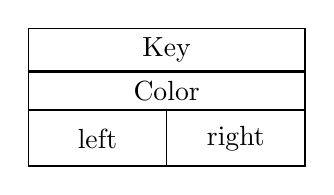
\begin{tikzpicture}
  \node (Key) [rectangle,draw,minimum width=10em] {Key};
  \node (Color) [rectangle,draw,anchor=north,minimum width=10em] at (Key.south) {Color};
  \node (LeftChild) [rectangle,draw,anchor=north west,minimum width=5em,,minimum height=0.7cm] at ( Color.south west) {left};
  \node (RightChild) [rectangle,draw,anchor=north east,minimum width=5em,,minimum height=0.7cm] at (Color.south east) {right};
\end{tikzpicture}
\caption{Implementazione di un nodo di un albero R\&B}\label{fig:rb-node}
\end{figure}

\dfn{Alberi R-B}{
Un albero rosso e nero è un albero binario di ricerca che rispetta i seguenti vincoli:
\begin{enumerate}
\item Ogni nodo è colorato di rosso o di nero;
\item Ogni foglia è colorata di nero e non contiene dati. Queste foglie sono dette \textbf{foglie esterne} o \textbf{NIL};
\item La radice è nera;
\item Ogni nodo rosso ha solo figli neri;
\item Per ogni nodo $x$, ogni percorso da $x$ a un nodo NIL contiene lo stesso numero di nodi neri. Questa quantità è detta \textbf{altezza nera} di $x$ e viene indicata con $bh(x)$.
\end{enumerate}
}

La Figura~\ref{fig:rb-tree} mostra un esempio di albero rosso-nero. In questo caso, il numero di nodi neri lungo ogni percorso da un nodo a una foglia esterna è sempre 3. È facile osservare che tutti gli alberi AVL possono essere alberi rossi e neri, secondo un'opportuna colorazione, ma non tutti gli alberi rossi e neri possono essere degli alberi AVL. Si consideri l'albero mostrato in Figura~\ref{fig:rb-not-avl}. Questo albero è un albero rosso nero in quanto rispetta ogni proprietà, ma non è un albero AVL in quanto la differenza di altezza tra il sottoalbero sinistro e quello destro del nodo $x$ è maggiore di 1. In Figura~\ref{fig:gerarchia-alberi} è mostrata la gerarchia degli alberi binari di ricerca perfettamente bilanciati, AVL e rossi e neri.

\begin{figure}[ht!]
\centering
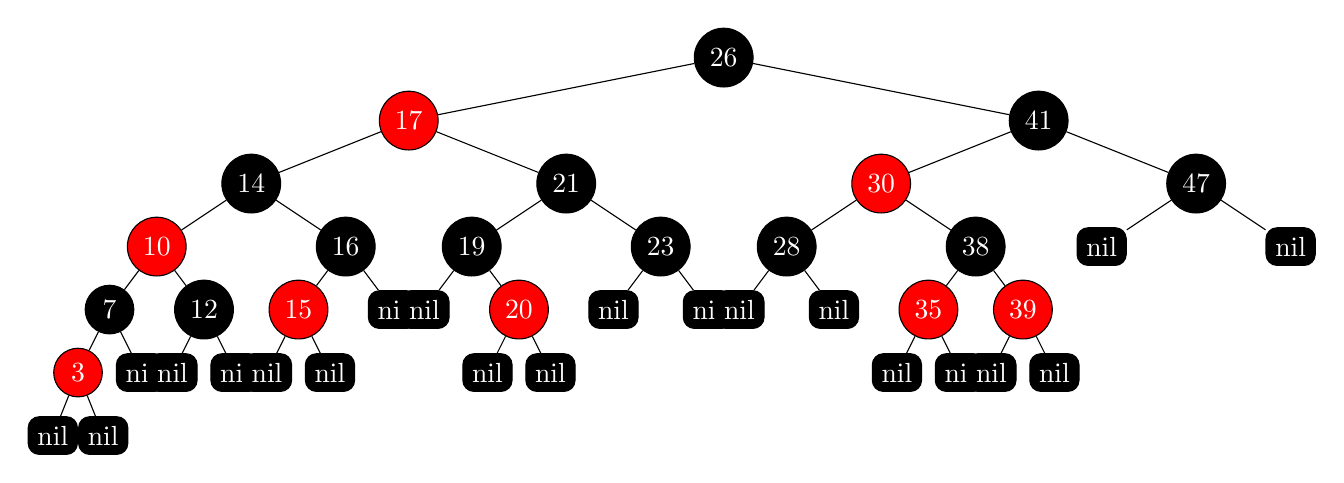
\begin{tikzpicture}
[level 1/.style={level distance=1cm, sibling distance=10cm},
level 2/.style={sibling distance=5cm},
level 3/.style={sibling distance=3cm},
level 4/.style={sibling distance=1.5cm},
level 5/.style={sibling distance=1cm},
level 6/.style={sibling distance=0.8cm},
root/.style={circle,draw,fill=black,text=white,minimum size=0.5cm},
rednode/.style={circle,draw,fill=red,text=white,minimum size=0.5cm},
blacknode/.style={circle,draw,fill=black,text=white,minimum size=0.5cm},
leaf/.style={rectangle,rounded corners,draw,fill=black,text=white,minimum height = 2mm, minimum width = 2mm},scale=0.8]
\node[root]{26}
child {
  node[rednode]{17}
    child{
      node[blacknode]{14}
      child{
        node[rednode]{10}
        child{
          node[blacknode]{7}
          child{
            node[rednode]{3}
            child{
              node[leaf]{nil}
            }
            child{
              node[leaf]{nil}
            }
          }
          child{
            node[leaf]{nil}
          }
        }
        child{
          node[blacknode]{12}
          child{
            node[leaf]{nil}
          }
          child{
            node[leaf]{nil}
          }
        }
      }
      child{
        node[blacknode]{16}
        child{
          node[rednode]{15}
          child{
            node[leaf]{nil}
          }
          child{
            node[leaf]{nil}
          }
        }
        child{
          node[leaf]{nil}
        }
      }
    }
    child{
      node[blacknode]{21}
      child{
        node[blacknode]{19}
        child{
          node[leaf]{nil}
        }
        child{
          node[rednode]{20}
          child{
            node[leaf]{nil}
          }
          child{
            node[leaf]{nil}
          }
        }
      }
      child{
        node[blacknode]{23}
        child{
          node[leaf]{nil}
        }
        child{
          node[leaf]{nil}
        }
      }
    }
}
child{
  node[blacknode]{41}
  child{
    node[rednode]{30}
    child{
      node[blacknode]{28}
      child{
        node[leaf]{nil}
      }
      child{
        node[leaf]{nil}
      }
    }
    child{
      node[blacknode]{38}
      child{
        node[rednode]{35}
        child{
          node[leaf]{nil}
        }
        child{
          node[leaf]{nil}
        }
      }
      child{
        node[rednode]{39}
        child{
          node[leaf]{nil}
        }
        child{
          node[leaf]{nil}
        }
      }
    }
  }
  child{
    node[blacknode]{47}
    child{
      node[leaf]{nil}
    }
    child{
      node[leaf]{nil}
    }
  }
};
\end{tikzpicture}
\caption{Albero rosso e nero}\label{fig:rb-tree}
\end{figure}

\begin{figure}[ht!]
\centering
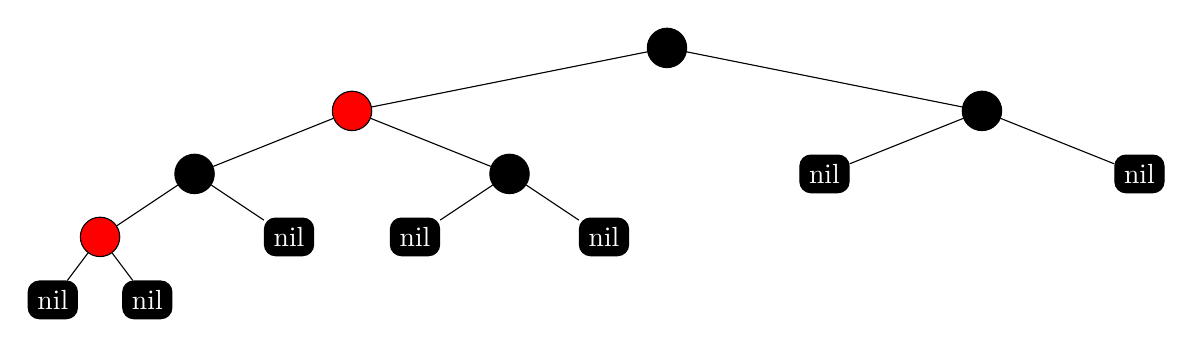
\begin{tikzpicture}
[level 1/.style={level distance=1cm, sibling distance=10cm},
level 2/.style={sibling distance=5cm},
level 3/.style={sibling distance=3cm},
level 4/.style={sibling distance=1.5cm},
level 5/.style={sibling distance=1cm},
level 6/.style={sibling distance=0.8cm},
root/.style={circle,draw,fill=black,text=white,minimum size=0.5cm},
rednode/.style={circle,draw,fill=red,text=white,minimum size=0.5cm},
blacknode/.style={circle,draw,fill=black,text=white,minimum size=0.5cm},
leaf/.style={rectangle,rounded corners,draw,fill=black,text=white,minimum height = 2mm, minimum width = 2mm},scale=.8]
\node[root]{}
child{
  node[rednode]{}
  child{
    node[blacknode]{}
    child{
      node[rednode]{}
      child{
        node[leaf]{nil}
      }
      child{
        node[leaf]{nil}
      }
    }
    child{
      node[leaf]{nil}
    }
  }
  child{
    node[blacknode]{}
    child{
      node[leaf]{nil}
    }
    child{
      node[leaf]{nil}
    }
  }
}
child{
  node[blacknode]{}
  child{
    node[leaf]{nil}
  }
  child{
    node[leaf]{nil}
  }
};
\end{tikzpicture}
\caption{Albero rosso e nero che non è un albero AVL}\label{fig:rb-not-avl}
\end{figure}


\begin{osservation}
Come si evince dal diagramma mostrato in Figura~\ref{fig:gerarchia-alberi} un albero pieno può essere colorabile come un albero rosso e nero. Un modo per colorarlo, infatti, è fare tutti i suoi nodi di nero. Questo perché gli alberi pieni hanno tutti i livelli saturi e di conseguenza tutti i percorsi da qualche nodo a una foglia avranno la stessa lunghezza. Un altro modo per colorarlo è alternando un livello rosso con un livello nero. Questo perché, essendo l'albero pieno, tutti i nodi di un livello hanno lo stesso numero di figli e, quindi, tutti i percorsi da qualche nodo a una foglia avranno la stessa lunghezza.
\end{osservation}


Non tutti gli alberi, però, sono colorabili. Sia ad esempio $T$ un albero binario come mostrato in Figura~\ref{fig:tree-not-colorable}. Da come si vede da questo esempio, nonostante i vincoli definiti per gli alberi rosso neri siano meno restrittivi di quanto visto per gli alberi AVL e APB, non tutti gli alberi binari di ricerca possono essere colorati come alberi rossi e neri. In particolare, un altro esempio di albero non colorabile è dato dalla classe degli alberi degeneri.

\begin{figure}[ht!]
\centering
\subfloat[\label{fig:tree-not-colorable}]{
	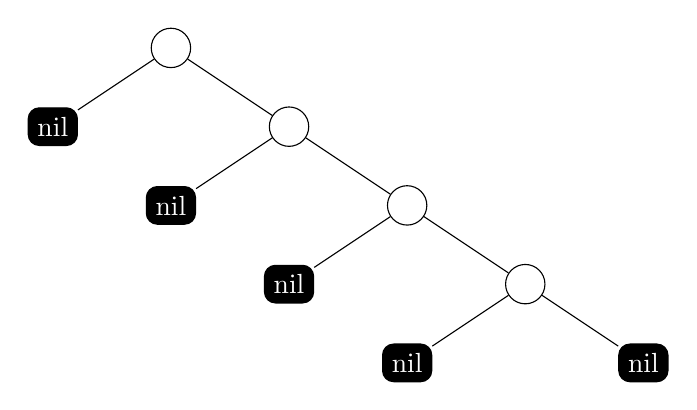
\begin{tikzpicture}
		[
		level 1/.style={level distance=1cm, sibling distance=3cm},
		level 2/.style={sibling distance=3cm},
		level 3/.style={sibling distance=3cm},
		level 4/.style={sibling distance=3cm},
		level 5/.style={sibling distance=3cm},
		level 6/.style={sibling distance=3cm},
		mynode/.style={
			circle,
			draw,
			minimum size=0.5cm
		},
		leaf/.style={rectangle,rounded corners,draw,fill=black,text=white,minimum height = 2mm, minimum width = 2mm}]
		\node[mynode]{}
		child{
			node[leaf]{nil}
		}
		child
		{
			node[mynode]{}
			child{
				node[leaf]{nil}
			}
			child{
				node[mynode]{}
				child{
					node[leaf]{nil}
				}
				child{
					node[mynode]{}
					child{
						node[leaf]{nil}
					}
					child{
						node[leaf]{nil}
					}
				}
			}
		};
\end{tikzpicture}} \qquad
\subfloat[Il colore della radice è ininfluente. Se è rossa, allora per il vincolo 3 il figlio dovrà essere nero. Così facendo notiamo però che il vincolo 4 non è rispettato. Il percorso che dalla radice arriva alla foglia ha un solo nodo nero, mentre il percorso che arriva alla foglia successiva ne ha due.]{
	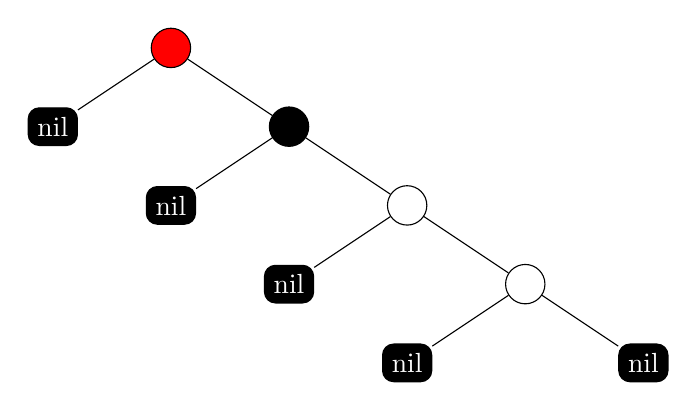
\begin{tikzpicture}
		[level 1/.style={level distance=1cm, sibling distance=3cm},
		level 2/.style={sibling distance=3cm},
		level 3/.style={sibling distance=3cm},
		level 4/.style={sibling distance=3cm},
		level 5/.style={sibling distance=3cm},
		level 6/.style={sibling distance=3cm},
		mynode/.style={
			circle,
			draw,
			minimum size=0.5cm
		},
		leaf/.style={rectangle,rounded corners,draw,fill=black,text=white,minimum height = 2mm, minimum width = 2mm}]
		\node[mynode,fill=red]{}
		child{
			node[leaf]{nil}
		}
		child
		{
			node[mynode,fill=black]{}
			child{
				node[leaf]{nil}
			}
			child{
				node[mynode]{}
				child{
					node[leaf]{nil}
				}
				child{
					node[mynode]{}
					child{
						node[leaf]{nil}
					}
					child{
						node[leaf]{nil}
					}
				}
			}
		};
	\end{tikzpicture}
} \\
\subfloat[Proviamo quindi a colorare la radice di nero. Il colore del figlio destro a questo punto non potrà essere che rosso se non si vuole squilibrare l'albero vioando il vincolo 5.]{
	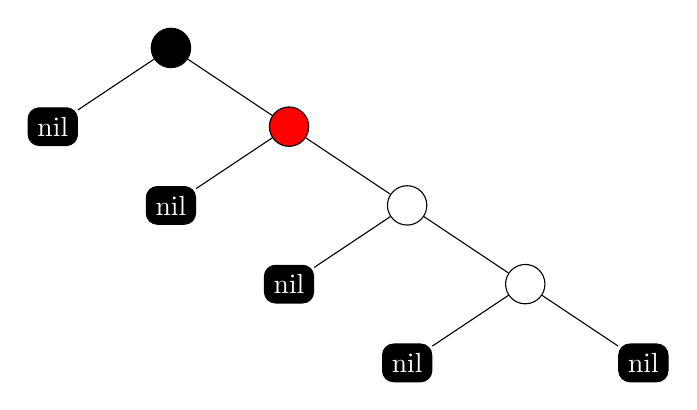
\begin{tikzpicture}
		[level 1/.style={level distance=1cm, sibling distance=3cm},
		level 2/.style={sibling distance=3cm},
		level 3/.style={sibling distance=3cm},
		level 4/.style={sibling distance=3cm},
		level 5/.style={sibling distance=3cm},
		level 6/.style={sibling distance=3cm},
		mynode/.style={
			circle,
			draw,
			minimum size=0.5cm
		},
		leaf/.style={rectangle,rounded corners,draw,fill=black,text=white,minimum height = 2mm, minimum width = 2mm}]
		\node[mynode,fill=black]{}
		child{
			node[leaf]{nil}
		}
		child
		{
			node[mynode,fill=red]{}
			child{
				node[leaf]{nil}
			}
			child{
				node[mynode]{}
				child{
					node[leaf]{nil}
				}
				child{
					node[mynode]{}
					child{
						node[leaf]{nil}
					}
					child{
						node[leaf]{nil}
					}
				}
			}
		};
\end{tikzpicture}} \qquad
\subfloat[Poiché si è colorato il secondo nodo di rosso, per il vincolo 4 il suo figlio dovrà essere nero. A questo punto però il vincolo 5 non è rispettato. Il percorso che dalla radice arriva alla foglia ha un solo nodo nero, mentre il percorso che arriva alla foglia successiva ne ha due.]{
	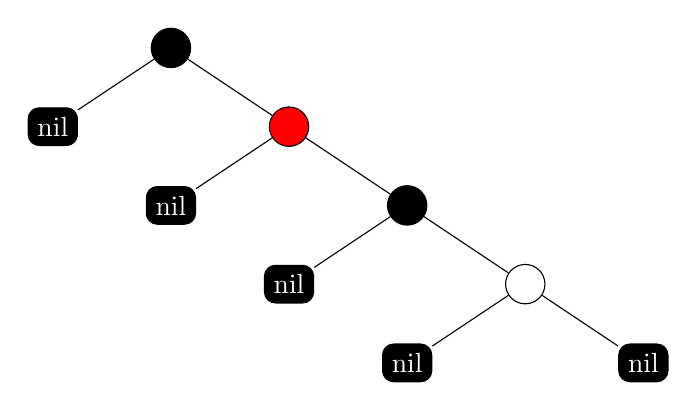
\begin{tikzpicture}
		[level 1/.style={level distance=1cm, sibling distance=3cm},
		level 2/.style={sibling distance=3cm},
		level 3/.style={sibling distance=3cm},
		level 4/.style={sibling distance=3cm},
		level 5/.style={sibling distance=3cm},
		level 6/.style={sibling distance=3cm},
		mynode/.style={
			circle,
			draw,
			minimum size=0.5cm
		},
		leaf/.style={rectangle,rounded corners,draw,fill=black,text=white,minimum height = 2mm, minimum width = 2mm}]
		\node[mynode,fill=black]{}
		child{
			node[leaf]{nil}
		}
		child
		{
			node[mynode,fill=red]{}
			child{
				node[leaf]{nil}
			}
			child{
				node[mynode,fill=black]{}
				child{
					node[leaf]{nil}
				}
				child{
					node[mynode]{}
					child{
						node[leaf]{nil}
					}
					child{
						node[leaf]{nil}
					}
				}
			}
		};
	\end{tikzpicture}
}
\caption{}
\end{figure}

\begin{center}
\begin{tikzpicture}[font=\tiny,scale=.7]
	\draw (0,0) [fill=primary!30]
	circle  (1cm)
	node {Alberi pieni}

	circle (2cm)
	node [align=center, anchor=north, yshift=1.2cm]{APB}

	circle (3cm)
	node [align=center, anchor=north, yshift=2cm]{Alberi AVL}

	circle (4cm)
	node [align=center, anchor=north, yshift=2.6cm]{Alberi R\&B}
	;
\end{tikzpicture}
\captionof{figure}{Relazione tra alberi perfettamente bilanciati, AVL e R\&B}\label{fig:gerarchia-alberi}
\end{center}

\subsection{Altezza di un albero rosso-nero}
I vincoli imposti sui nodi di un albero rosso-nero garantiscono che l'altezza dell'albero sia logaritmica sul numero dei nodi. In particolare, vincolare ogni nodo rosso ad avere solo figli neri e fissare l'altezza nera di ogni nodo a $bh(x)$, garantisce il contenimento dell'altezza dell'albero.


\begin{lemmabox}
Il numero di nodi interni di un sottoalbero radicato in $x$ è maggiore o uguale di $2^{bh(x)}-1$.
\end{lemmabox}
\begin{proof}
Si dimostra per induzione sull'altezza $h(x)$ dell'albero radicato in $x$:

\begin{itemize}
\item \textbf{Caso base:} $h(x)=0$. In questo caso, $x$ è una foglia esterna e, per definizione, non ha figli. Il numero di nodi interni è quindi $0$ e $2^{bh(x)}-1=2^0-1=0$.

\item \textbf{Passo induttivo:} $h(x)>0$. In questo caso, $x$ è un nodo interno e ha due figli: $s$ e $d$. Qual è la loro altezza nera? Distinguiamo due casi:
\begin{itemize}
\item $s$ è rosso. Allora $bh(s)=bh(x)\geq bh(x)-1$;
\item $s$ è nero. Allora $bh(s)=bh(x)-1\geq bh(x)-1$.
\end{itemize}
In maniera analoga abbiamo che $bh(d)\geq bh(x)-1$. Il numero dei nodi interni radicato in $x$ sarà pari a:
\begin{displaymath}
1 + \#_{int}(s) + \#_{int}(d)
\end{displaymath}
Poiché $h(s),h(d)<h(x)$ possiamo applicare l'ipotesi induttiva e ottenere:
\begin{displaymath}
\#_{int}(s)\geq 2^{bh(s)}-1 \geq 2^{bh(x)-1}-1
\end{displaymath}
e
\begin{displaymath}
\#_{int}(d)\geq 2^{bh(d)}-1 \geq 2^{bh(x)-1}-1
\end{displaymath}
Allora:
\begin{eqnarray*}
\#_{int}(x) &=& 1 + \#_{int}(s) + \#_{int}(d) \\
&\geq& 1 + 2 \cdot \bigl( 2^{bh(x)-1}-1\bigr) \\
&=& 2^{bh(x)}-1
\end{eqnarray*}
\end{itemize}
\end{proof}



\begin{teorbox}
L'altezza massima di un albero rosso-nero con $n$ nodi è al più $2\log(n+1)$.
\end{teorbox}
\begin{proof}
Sia $h$ l'altezza dell'albero. Per il vincolo 5, in ogni percorso da un nodo ad una foglia almeno la metà dei nodi sono neri. Allora, l'altezza nera dell'albero dovrà essere almeno $h/2$. Per il Lemma precedente, il numero di nodi interni dell'albero è almeno $2^{bh(T)}-1$. Allora:
\begin{center}
$\renewcommand\arraystretch{2}
\begin{array}{lll}
n & \geq 2^{bh(T)}-1 & \textcolor{gray}{\text{(per il Lemma precedente)}} \\
& \geq 2^{h/2}-1 & \textcolor{gray}{\text{(per il vincolo 5)}} \\
n+1 & \geq 2^{h/2} & \textcolor{gray}{\text{(spostando l'1 al primo membro)}} \\
\log(n+1) & \geq \frac{h}{2} & \textcolor{gray}{\text{(applicando il logaritmo)}} \\
2\log(n+1) & \geq h & \textcolor{gray}{\text{(moltiplicando per 2)}}
\end{array}$
\end{center}

In questo modo abbiamo trovato un limite superiore all'altezza dell'albero che dimostra il buon bilanciamento dell'albero.
\end{proof}

\begin{corolbox}
In un albero rosso nero le operazioni di ricerca, inserimento e cancellazione hanno un costo logaritmico sul numero dei nodi.
\end{corolbox}

\subsection{Inserimento in un albero rosso-nero}
L'inserimento in un albero rosso-nero è simile all'inserimento in un albero binario di ricerca. Esattamente come per gli alberi binari di ricerca, l'algoritmo di inserimento di un nodo $z$ in un albero rosso-nero cerca un cammino discendente dalla radice dell'albero fino al nodo $y$ che ne diventerà padre.

Una volta identificato il nodo $y$, il nodo $x$ viene inserito come figlio sinistro di $y$ se $z\rightarrow key \leq y \rightarrow key$, destro altrimenti. Tuttavia, nel caso di alberi rosso-neri bisognerà risolvere il problema di mantenere i vincoli imposti sui nodi dell'albero. In particolare, l'inserimento di un nodo potrebbe violare il vincolo 5, che impone che tutti i cammini da un qualsiasi nodo alle foglie sue discendenti abbiano lo stesso numero di nodi neri. Per questo motivo, l'inserimento di un nodo implicherebbe una sua colorazione di rosso. Tuttavia, questa colorazione potrebbe violare il vincolo 4, che impone che ogni nodo rosso abbia solo figli neri.

In generale, l'inserimento di un nodo potrebbe richiedere una serie di rotazioni e ricolorazioni dei nodi dell'albero. L'idea alla base per il ripristino della proprietà red-black, se necessario, al ritorno dalle chiamate ricorsive presenti nell'Algoritmo~\ref{lst:insert-rb} è la seguente: spostare le violazioni verso l'alto rispettando sempre il vincolo 5. Se la violazione arriva alla radice, la coloriamo di nero. Così facendo le operazioni di ripristino saranno necessarie solo quando due nodi consecutivi risultano rossi. In Figura~\ref{fig:rb-insertion} è mostrato un esempio di inserimento di un nodo in un albero rosso-nero.


\begin{lstlisting}[language=asd,caption={Insert-RB(T,k)},label=lst:insert-rb]
if not IS-NIL(T) then
if T@\rightarrow@ key < k then
T@\rightarrow@ right = Insert-RB(T@\rightarrow@ right,k)
T = Bilancia-Destra-RB(T)
else if T@\rightarrow@ key > k then
T@\rightarrow@ left = Insert-RB(T@\rightarrow@ left,k)
T = Bilancia-Sinistra-RB(T)
else
T = NewNodeRB(k)
T@\rightarrow@ color = RED
return T
\end{lstlisting}

\begin{center}
\begin{minipage}{.9\textwidth}
\centering
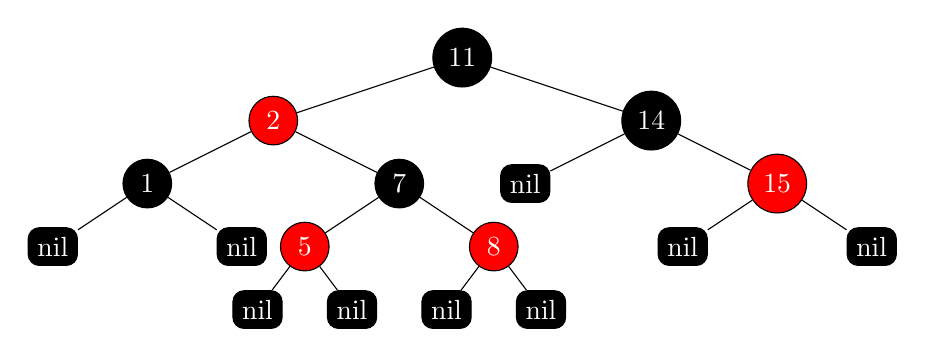
\begin{tikzpicture}
[scale=.8,
level 1/.style={level distance=1cm, sibling distance=6cm},
level 2/.style={sibling distance=4cm},
level 3/.style={sibling distance=3cm},
level 4/.style={sibling distance=1.5cm},
level 5/.style={sibling distance=1cm},
root/.style={circle,draw,fill=black,text=white,minimum size=0.5cm},
rednode/.style={circle,draw,fill=red,text=white,minimum size=0.5cm},
blacknode/.style={circle,draw,fill=black,text=white,minimum size=0.5cm},
leaf/.style={rectangle,rounded corners,draw,fill=black,text=white,minimum height = 2mm, minimum width = 2mm}]
\node[root]{11}
child{
  node[rednode]{2}
  child{
    node[blacknode]{1}
    child{
      node[leaf]{nil}
    }
    child{
      node[leaf]{nil}
    }
  }
  child{
    node[blacknode]{7}
    child{
      node[rednode]{5}
      child{
        node[leaf]{nil}
      }
      child{
        node[leaf]{nil}
      }
    }
    child{
      node[rednode]{8}
      child{
        node[leaf]{nil}
      }
      child{
        node[leaf]{nil}
      }
    }
  }
}
child{
  node[blacknode]{14}
  child{
    node[leaf]{nil}
  }
  child{
    node[rednode]{15}
    child{
      node[leaf]{nil}
    }
    child{
      node[leaf]{nil}
    }
  }
};
\end{tikzpicture}
\captionof{figure}{Albero dove inserire il nodo $z$\label{fig:rb-insertion}}
\end{minipage}
\\
\begin{minipage}{.9\textwidth}
\centering
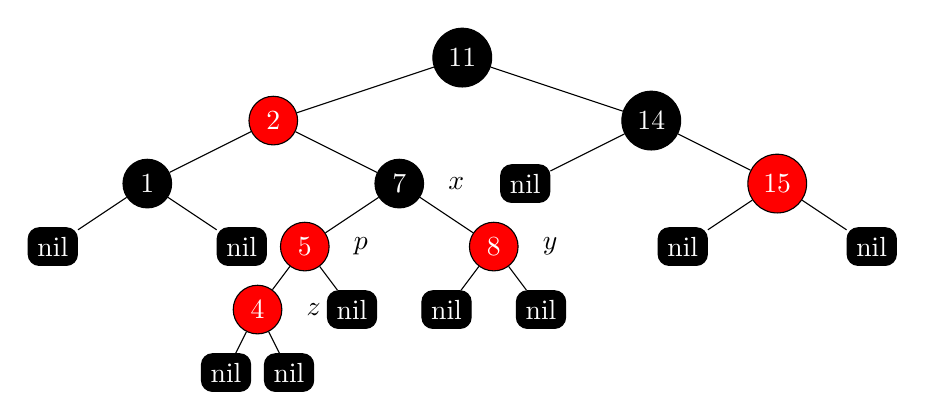
\begin{tikzpicture}
[scale=.8,
level 1/.style={level distance=1cm, sibling distance=6cm},
level 2/.style={sibling distance=4cm},
level 3/.style={sibling distance=3cm},
level 4/.style={sibling distance=1.5cm},
level 5/.style={sibling distance=1cm},
root/.style={circle,draw,fill=black,text=white,minimum size=0.5cm},
rednode/.style={circle,draw,fill=red,text=white,minimum size=0.5cm},
blacknode/.style={circle,draw,fill=black,text=white,minimum size=0.5cm},
leaf/.style={rectangle,rounded corners,draw,fill=black,text=white,minimum height = 2mm, minimum width = 2mm}]
\node[root]{11}
child{
  node[rednode]{2}
  child{
    node[blacknode]{1}
    child{
      node[leaf]{nil}
    }
    child{
      node[leaf]{nil}
    }
  }
  child{
    node[blacknode,name=x]{7}
    child{
      node[rednode,name=p]{5}
      child{
        node[rednode,name=z]{4}
        child{
          node[leaf]{nil}
        }
        child{
          node[leaf]{nil}
        }
      }
      child{
        node[leaf]{nil}
      }
    }
    child{
      node[rednode,name=y]{8}
      child{
        node[leaf]{nil}
      }
      child{
        node[leaf]{nil}
      }
    }
  }
}
child{
  node[blacknode]{14}
  child{
    node[leaf]{nil}
  }
  child{
    node[rednode]{15}
    child{
      node[leaf]{nil}
    }
    child{
      node[leaf]{nil}
    }
  }
};
\node[right,xshift=0.5cm] at (y) {$y$};
\node[right,xshift=0.5cm] at (x) {$x$};
\node[right,xshift=0.5cm] at (z) {$z$};
\node[right,xshift=0.5cm] at (p) {$p$};
\end{tikzpicture}
\captionof{figure}{L'inserimento del nodo $z$ causa una violazione del vincolo 4. Per risolvere il problema, il nodo $y$ viene ricolorato di nero e il suo genitore $x$ di rosso.}
\end{minipage}
\\
\begin{minipage}{.9\textwidth}
\centering
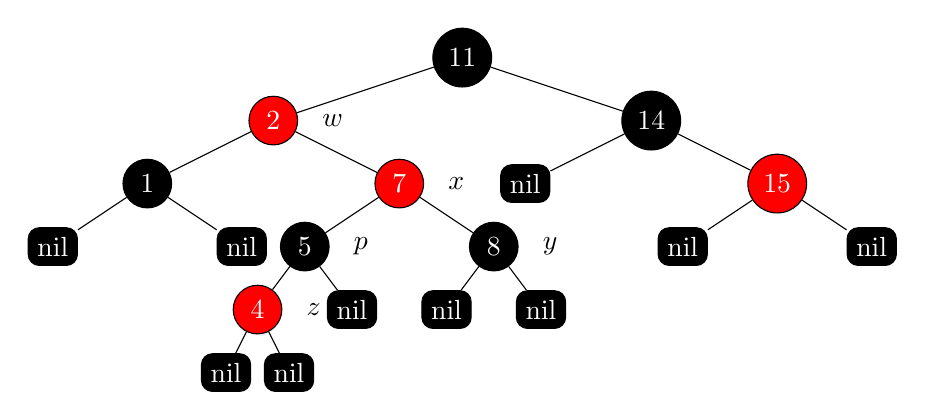
\begin{tikzpicture}
[scale=.8,
level 1/.style={level distance=1cm, sibling distance=6cm},
level 2/.style={sibling distance=4cm},
level 3/.style={sibling distance=3cm},
level 4/.style={sibling distance=1.5cm},
level 5/.style={sibling distance=1cm},
root/.style={circle,draw,fill=black,text=white,minimum size=0.5cm},
rednode/.style={circle,draw,fill=red,text=white,minimum size=0.5cm},
blacknode/.style={circle,draw,fill=black,text=white,minimum size=0.5cm},
leaf/.style={rectangle,rounded corners,draw,fill=black,text=white,minimum height = 2mm, minimum width = 2mm}]
\node[root]{11}
child{
  node[rednode,name=w]{2}
  child{
    node[blacknode]{1}
    child{
      node[leaf]{nil}
    }
    child{
      node[leaf]{nil}
    }
  }
  child{
    node[rednode,name=x]{7}
    child{
      node[blacknode,name=p]{5}
      child{
        node[rednode,name=z]{4}
        child{
          node[leaf]{nil}
        }
        child{
          node[leaf]{nil}
        }
      }
      child{
        node[leaf]{nil}
      }
    }
    child{
      node[blacknode,name=y]{8}
      child{
        node[leaf]{nil}
      }
      child{
        node[leaf]{nil}
      }
    }
  }
}
child{
  node[blacknode]{14}
  child{
    node[leaf]{nil}
  }
  child{
    node[rednode]{15}
    child{
      node[leaf]{nil}
    }
    child{
      node[leaf]{nil}
    }
  }
};
\node[right,xshift=0.5cm] at (y) {$y$};
\node[right,xshift=0.5cm] at (x) {$x$};
\node[right,xshift=0.5cm] at (z) {$z$};
\node[right,xshift=0.5cm] at (p) {$p$};
\node[right,xshift=0.5cm] at (w) {$w$};
\end{tikzpicture}
\captionof{figure}{In questo caso si procede con la ricolorazione del nodo $p$ e $y$ da rossi a neri mentre il nodo $x$ diventa nero per non alterare il numero di nodi neri. A  questo punto però si viola il vincolo 4 sul nodo $w$. Per risolvere lo sbilanciamento sarà quindi necessario cambiare il colore di $x$ e della radice violando così il vincolo 2 per evitare di violare il vincolo 5. Sarà quindi necessario procedere con una rotazione a destra per ripristinare il vincolo 2.}
\end{minipage}
\\
\begin{minipage}{.9\textwidth}
\centering
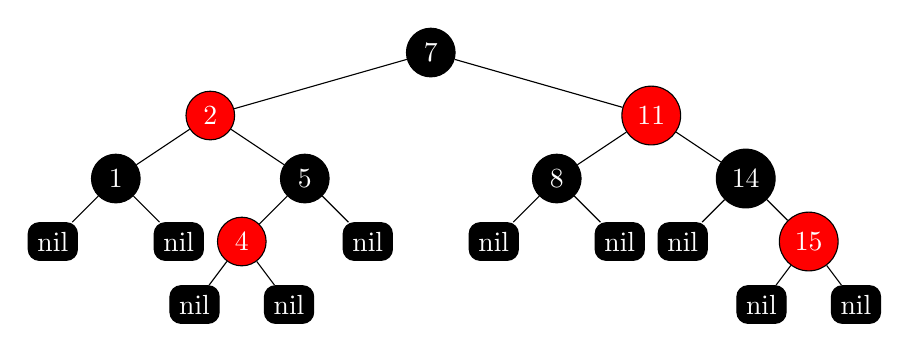
\begin{tikzpicture}
[scale=.8,
level 1/.style={level distance=1cm, sibling distance=7cm},
level 2/.style={sibling distance=3cm},
level 3/.style={sibling distance=2cm},
level 4/.style={sibling distance=1.5cm},
level 5/.style={sibling distance=1cm},
root/.style={circle,draw,fill=black,text=white,minimum size=0.5cm},
rednode/.style={circle,draw,fill=red,text=white,minimum size=0.5cm},
blacknode/.style={circle,draw,fill=black,text=white,minimum size=0.5cm},
leaf/.style={rectangle,rounded corners,draw,fill=black,text=white,minimum height = 2mm, minimum width = 2mm}
]
\node[root]{7}
child{
 node[rednode]{2}
 child{
  node[blacknode]{1}
  child{
   node[leaf]{nil}
  }
  child{
   node[leaf]{nil}
  }
 }
 child{
  node[blacknode]{5}
  child{
    node[rednode]{4}
    child{
      node[leaf]{nil}
    }
    child{
      node[leaf]{nil}
    }
  }
  child{
    node[leaf]{nil}
  }
 }
}
child{
  node[rednode]{11}
  child{
    node[blacknode]{8}
    child{
      node[leaf]{nil}
    }
    child{
      node[leaf]{nil}
    }
  }
  child{
    node[blacknode]{14}
    child{
      node[leaf]{nil}
    }
    child{
      node[rednode]{15}
      child{
        node[leaf]{nil}
      }
      child{
        node[leaf]{nil}
      }
    }
  }
};
\end{tikzpicture}
\captionof{figure}{Albero finale}
\end{minipage}
\end{center}

\subsubsection{Il bilanciamento del sottoalbero sinistro}
Come detto in precedenza, le operazioni di ripristino sono necessarie solo quando due nodi consecutivi sono rossi. Tra l'altro, se la radice dell'albero è sempre nera, non si presenterà mai la necessità di ribilanciare in un albero (o sottoalbero) di altezza minore di 3 in quanto non si possono verificare violazioni. A fronte di queste osservazioni possiamo distinguere tre casi possibili che possono scatenare una violazione del vincolo 4 a fronte dell'inserimento di un nuovo nodo $z$:
\begin{enumerate}
\item Lo zio $y$ di $z$ è rosso (Figura~\ref{fig:rb-insertion-case1});
\item Lo zio $y$ di $z$ è nero e $z$ è il figlio destro del figlio sinistro del padre $p$ (Figura~\ref{fig:rb-insertion-case2});
\item Lo zio $y$ di $z$ è nero e $z$ è il figlio sinistro del figlio sinistro del padre $p$ (Figura~\ref{fig:rb-insertion-case3}).
\end{enumerate}
L'Algoritmo \textsc{Bilancia-Sinistra-RB} (Algoritmo \ref{lst:bilancia-sx-rb}) sulla base di questi tre casi, provvede a ripristinare la proprietà red-black dell'albero. Con al massimo due rotazioni si riesce a risolvere il problema di bilanciamento. Questo però non deve stupire in quanto gli alberi rosso-neri sono più tolleranti degli alberi AVL e quindi è normale che ci siano meno rotazioni. Il vantaggio computazionale degli alberi rosso-neri rispetto agli alberi AVL sarà ben visibile nella fase di cancellazione. L'Algoritmo \textsc{Tipo-Violazione-Sinistra} (Algoritmo \ref{lst:tipo-violazione-sx}) calcola il tipo di violazione che si è verificata.

\begin{lstlisting}[language=asd,caption={Bilancia-Sinistra-RB(T)},label=lst:bilancia-sx-rb]
if ha_figlio(T@\rightarrow@left)
v = Tipo-Violazione_Sinistra(T@\rightarrow@left,T@\rightarrow@right)
case v of
1: T = Caso1(T)
2: T = Caso2(T)
3: T = Caso3(T)
return T
\end{lstlisting}


\begin{lstlisting}[language=asd,caption={Tipo-Violazione-Sinistra(S,D)},label=lst:tipo-violazione-sx]
v = 0
if S@\rightarrow@color = RED && D@\rightarrow@ color = RED then
if S@\rightarrow@left@\rightarrow@color = RED || S@\rightarrow@right@\rightarrow@color=R then
v = 1
else
if S@\rightarrow@color = RED && S@\rightarrow@right@\rightarrow@color = RED then
v = 2
else
if S@\rightarrow@left@\rightarrow@color = RED then
v = 3
return v
\end{lstlisting}

\begin{figure}[ht!]
\centering
\subfloat[Caso 1\label{fig:rb-insertion-case1}]
{
	\begin{tikzpicture}
		[
		level 1/.style={level distance=1cm, sibling distance=6cm},
		level 2/.style={sibling distance=4cm},
		level 3/.style={sibling distance=3cm},
		level 4/.style={sibling distance=1.5cm},
		level 5/.style={sibling distance=1cm},
		root/.style={circle,draw,fill=black,text=white,minimum size=0.5cm},
		rednode/.style={circle,draw,fill=red,text=white,minimum size=0.5cm},
		blacknode/.style={circle,draw,fill=black,text=white,minimum size=0.5cm},
		leaf/.style={rectangle,rounded corners,draw,fill=black,text=white,minimum height = 2mm, minimum width = 2mm},
		itria/.style={
			draw,
			shape border uses incircle,
			isosceles triangle,
			shape border rotate=90,
			yshift=-0.5cm
		},scale=.7]
		\node[blacknode]{C}
		child{
			node[rednode]{A}
			child{
				node[circle,fill=black]{}{node[itria]{}}
			}
			child{
				node[rednode,name=x]{B}
				child{
					node[circle,fill=black]{}{node[itria]{}}
				}
				child{
					node[circle,fill=black]{}{node[itria]{}}
				}
			}
		}
		child{
			node[rednode,name=y]{D}
			child{
				node[circle,fill=black]{}{node[itria]{}}
			}
			child{
				node[circle,fill=black]{}{node[itria]{}}
			}
		};
		\node[right,xshift=0.5cm] at (x) {$z$};
		\node[right,xshift=0.5cm] at (y) {$y$};
	\end{tikzpicture}
} \hfil
\subfloat[Caso 2\label{fig:rb-insertion-case2}]{
	\begin{tikzpicture}
		[
		level 1/.style={level distance=1cm, sibling distance=6cm},
		level 2/.style={sibling distance=4cm},
		level 3/.style={sibling distance=3cm},
		level 4/.style={sibling distance=1.5cm},
		level 5/.style={sibling distance=1cm},
		root/.style={circle,draw,fill=black,text=white,minimum size=0.5cm},
		rednode/.style={circle,draw,fill=red,text=white,minimum size=0.5cm},
		blacknode/.style={circle,draw,fill=black,text=white,minimum size=0.5cm},
		leaf/.style={rectangle,rounded corners,draw,fill=black,text=white,minimum height = 2mm, minimum width = 2mm},
		itria/.style={
			draw,
			shape border uses incircle,
			isosceles triangle,
			shape border rotate=90,
			yshift=-0.5cm
		},scale=.7]
		\node[blacknode]{C}
		child{
			node[rednode]{A}
			child{
				node[circle,fill=black]{}{node[itria]{}}
			}
			child{
				node[rednode,name=x]{B}
				child{
					node[circle,fill=black]{}{node[itria]{}}
				}
				child{
					node[circle,fill=black]{}{node[itria]{}}
				}
			}
		}
		child{
			node[circle,fill=black]{}{node[itria,fill=black,name=y]{}}
		};
		\node[right,xshift=0.5cm] at (x) {$z$};
		\node[right,xshift=0.5cm] at (y) {$y$};
	\end{tikzpicture}
}\\
\subfloat[Caso 3\label{fig:rb-insertion-case3}]{
	\begin{tikzpicture}
		[
		level 1/.style={level distance=1cm, sibling distance=6cm},
		level 2/.style={sibling distance=4cm},
		level 3/.style={sibling distance=3cm},
		level 4/.style={sibling distance=1.5cm},
		level 5/.style={sibling distance=1cm},
		root/.style={circle,draw,fill=black,text=white,minimum size=0.5cm},
		rednode/.style={circle,draw,fill=red,text=white,minimum size=0.5cm},
		blacknode/.style={circle,draw,fill=black,text=white,minimum size=0.5cm},
		leaf/.style={rectangle,rounded corners,draw,fill=black,text=white,minimum height = 2mm, minimum width = 2mm},
		itria/.style={
			draw,
			shape border uses incircle,
			isosceles triangle,
			shape border rotate=90,
			yshift=-0.5cm
		},scale=.7]
		\node[blacknode]{C}
		child{
			node[rednode]{B}
			child{
				node[rednode,name=x]{A}
				child{
					node[circle,fill=black]{}{node[itria]{}}
				}
				child{
					node[circle,fill=black]{}{node[itria]{}}
				}
			}
			child{
				node[circle,fill=black]{}{node[itria]{}}
			}
		}
		child{
			node[circle,fill=black]{}{node[itria,fill=black,name=y]{}}
		};
		\node[right,xshift=0.5cm] at (x) {$z$};
		\node[right,xshift=0.5cm] at (y) {$y$};
	\end{tikzpicture}
}
\caption{}
\end{figure}

\begin{minipage}{0.3\textwidth}
\begin{lstlisting}[language=asd,caption={Caso1(T)},label=lst:caso1-insert-rb]
T@\rightarrow@right@\rightarrow@color = BLACK
T@\rightarrow@left@\rightarrow@color = BLACK
T@\rightarrow@color = RED
return T
\end{lstlisting}
\end{minipage}\hfil
\begin{minipage}{0.35\textwidth}
\begin{lstlisting}[language=asd,caption={Caso2(T)},label=lst:caso2-insert-rb]
T@\rightarrow@left = Rotazione-Sx(T@\rightarrow@left)
T = Caso3(T)
return T
\end{lstlisting}
\end{minipage}\hfil
\begin{minipage}{0.3\textwidth}
\begin{lstlisting}[language=asd,caption={Caso3(T)},label=lst:caso3-insert-rb]
	T = Rotazione-Sx(T)
	T@\rightarrow@color = BLACK
	T@\rightarrow@right@\rightarrow@color = RED
	return T
\end{lstlisting}
\end{minipage}

\subsection{La cancellazione in un albero rosso-nero}
Analogamente ad altre operazioni elementari su un albero rosso-nero di $n$ nodi, la cancellazione di un nodo richiede un tempo logaritmico sul numero di nodi. A differenza però degli altri algoritmi di cancellazione, la cancellazione in un albero rosso-nero è più complessa in quanto richiede maggiori controlli per mantenere i vincoli imposti.



\begin{osservation}
Le operazioni di ripristino del bilanciamento sono necessarie solo quando il nodo cancellato è nero. Infatti, nel caso della cancellazione, non si può decidere a priori il colore del nodo da staccare. Qualora si dovesse eliminare un nodo nero siamo certi di aver modificato l'altezza nera dell'albero violando così il vincolo 5. Nel caso della cancellazione di un nodo rosso invece, si potrebbe al massimo aver avvicinato due nodi neri lungo un percorso ma la cosa non intacca alcun vincolo. Ripristinare questo vincolo però non è così complicato. L'idea alla base è quella di ignorare di aver violato il vincolo globale effettuando una \textbf{propagazione del colore nero} sul nodo che lo andrà a sostituire.
\end{osservation}


Se il nodo figlio era rosso allora è possibile colorarlo di nero, ma se questo fosse nero allora verrà colorato di un nuovo colore chiamato \textbf{doppio nero} (dal contributo che offre nel calcolo dell'altezza nera). In questo modo, il vincolo 5 verrà ripristinato. Tuttavia, questa introduzione di un terzo colore vìola il vincolo 1 che stabiliva che ogni nodo possa essere colorato o di rosso o di nero. Il problema per il ribilanciamento diventa quindi quello di eliminare i nodi doppio nero. L'algoritmo di cancellazione adotta una strategia simile a quella vista per la cancellazione negli alberi AVL.

\begin{minipage}{.45\textwidth}
\begin{lstlisting}[language=asd,caption={Delete-RB(T,k)},label=lst:delete-rb]
if !nil(T) then
if T@\rightarrow@ key < k then
T@\rightarrow@ right = Delete-RB(T@\rightarrow@ right,k)
T = Bilancia-Canc-Destra-RB(T)
else if T@\rightarrow@ key > k then
T@\rightarrow@ left = Delete-RB(T@\rightarrow@ left,k)
T = Bilancia-Canc-Sinistra-RB(T)
else
T = Delete-Root-RB(T)
return T
\end{lstlisting}

\begin{lstlisting}[language=asd,caption={Propagate-Black(T)},label=lst:propagate-black]
if T@\rightarrow@ color= RED then
T@\rightarrow@ color = BLACK
else
T@\rightarrow@ color = DOUBLE_BLACK
\end{lstlisting}
\end{minipage}
\hfil
\begin{minipage}{.4\textwidth}
\begin{lstlisting}[language=asd,caption={Delete-Root-RB(T)},label=lst:delete-root-rb]
if !nil(T) then
tmp = T
if nil(T@\rightarrow@ left) then
T = T @\rightarrow@ right
if tmp @\rightarrow@ color = BLACK then
  Propagate-Black(T)
else if nil(T@\rightarrow@ right) then
T = T@\rightarrow@ left
if tmp @\rightarrow@ color = BLACK then
  Propagate-Black(T)
else
tmp = Stacca-Min-RB(T@\rightarrow@ right,T)
T@\rightarrow@ key = tmp@\rightarrow@key
T = Bilancia-Canc-Destra-RB(T)
free(tmp)
return T
\end{lstlisting}
\end{minipage}

L'algoritmo \textsc{Stacca-Min-RB} è lo stesso visto per gli alberi AVL:
\begin{lstlisting}[language=asd,caption={Stacca-Min-RB(T,P)},label=lst:stacca-min-rb]
ret = nil
if !nil(P) && !nil(T) then
if !nil(T@\rightarrow@ left) then
ret = Stacca-Min-RB(T@\rightarrow@ left,T)
newT = Bilancia-Canc-Sinistra-RB(T)
else
ret = T
newT = T@\rightarrow@ right
if T @\rightarrow@ color = BLACK then
  Propagate-Black(newT)
if P @\rightarrow@ left = T then
  P @\rightarrow@ left = newT
else
  P @\rightarrow@ right = newT
return ret
\end{lstlisting}

\subsubsection{Il bilanciamento del sottoalbero sinistro}
Anche in questo caso, il bilanciamento del sottoalbero sinistro\footnote{Nel caso di sbilanciamento a destra si procede in modo simmetrico.} è simile a quello visto per gli alberi AVL. In particolare, l'algoritmo \textsc{Bilancia-Canc-Sinistra-RB} (Codice~\ref{lst:bilancia-sx-rb-del}) provvede a ripristinare la proprietà red-black dell'albero  eseguendo rotazioni e cambiamenti di colore. I vincoli che si possono violare a seguito della cancellazione di un nodo sono i seguenti:

\begin{itemize}
\item \textbf{Violazione del vincolo 3:} la radice può essere un nodo rosso;
\item \textbf{Violazione del vincolo 4:} se il padre e uno dei figli del nodo cancellato erano rossi;
\item \textbf{Violazione del vincolo 5:} altezza nera cambiata.
\end{itemize}

I casi che possono scatenare una violazione sono invece 4:
\begin{enumerate}
\item Il colore del fratello è rosso (Figura~\ref{fig:rb-deletion-case1});
\item I nipoti sono neri (Figura~\ref{fig:rb-deletion-case2});
\item Il nipote sinistro è rosso e il nipote destro è nero (Figura~\ref{fig:rb-deletion-case3});
\item Il nipote destro è rosso (Figura~\ref{fig:rb-deletion-case4}).
\end{enumerate}

\begin{lstlisting}[language=asd,caption={\textsc{Bilancia-Canc-Sinistra-RB}(T)},label=lst:bilancia-sx-rb-del]
if !nil(T@\rightarrow@ right) then
v = Violazione_Sx(T@\rightarrow@ left, T@\rightarrow@right)
case v of:
	1: T = Caso1(T)
 T = Bilancia-Canc-Sinistra(T@\rightarrow@left)
	2: T = Caso2(T)
	3: T = Caso3(T)
	4: T = Caso4(T)
return T
\end{lstlisting}

\begin{lstlisting}[language=asd,caption={\textsc{Violazione\_Sx}(X,W)},label=lst:violazione-sx]
	v = 0
	if X@\rightarrow@ color = DOUBLE-BLACK then
	if W@\rightarrow@ color = RED then
	v = 1
	else if W@\rightarrow@ right @\rightarrow@ color = BLACK && W @\rightarrow@ left @\rightarrow@ color = BLACK
	v = 2
	else if W@\rightarrow@ left @\rightarrow@ color = RED && W @\rightarrow@ right @\rightarrow@ color = BLACK
	v = 3
	else
	v = 4
	return v
\end{lstlisting}


Per comprendere il caso che effettua lo sbilanciamento si effettua un controllo sugli alberi del sottoalbero destro del padre del nodo doppio nero. Si ottiene così l'Algoritmo \textsc{Violazione-Sx} (Codice~\ref{lst:violazione-sx}). Analizziamo ora la gestione dei vari casi.

\paragraph{Caso 1:} il fratello è rosso. In questo caso, il fratello può essere colorato di nero e il padre può essere colorato di rosso. Successivamente si applica una rotazione destra sul fratello. A questo punto di determina una violazione sul nodo $E$ in quanto vede diminuita la sua altezza nera. Per risolvere la violazione del sottoalbero destro si ricolora la radice $D$ di nero ritrovandoci così nella situazione di una violazione del vincolo 5 nel sottoalbero sinistro. Quest'ultima violazione si risolve facilmente colorando il nodo $A$ di rosso. A questo punto ci si ritrova con un sottoalbero sbilanciato a sinistra di $A$ che è risolvibile riconducendosi al caso 2, 3 o 4.
\begin{lstlisting}[language=asd,caption={Caso1(T)},label=lst:caso1-rb-del]
T = Rotazione-Destra(T)
T@\rightarrow@ color = BLACK
T@\rightarrow@ right @\rightarrow@ color = RED
return T
\end{lstlisting}
\begin{figure}[ht!]
\centering
\subfloat[Configurazione iniziale\label{fig:rb-deletion-case1}]{
\begin{tikzpicture}
[
level 1/.style={level distance=1cm, sibling distance=6cm},
level 2/.style={sibling distance=4cm},
level 3/.style={sibling distance=3cm},
level 4/.style={sibling distance=1.5cm},
itria/.style={
draw,
dashed,
shape border uses incircle,
isosceles triangle,
shape border rotate=90,
yshift=-0.5cm,
fill=blue!25!white
},
root/.style={circle,draw,fill=black,text=white,minimum size=0.5cm},
rednode/.style={circle,draw,fill=red,text=white,minimum size=0.5cm},
blacknode/.style={circle,draw,fill=black,text=white,minimum size=0.5cm},
dbnode/.style={draw, circle, text centered, minimum size=0.5cm, fill=black, text=white, double,line width=2pt},
leaf/.style={rectangle,rounded corners,draw,fill=black,text=white,minimum height = 2mm, minimum width = 2mm},scale=.75
]
\node[root]{A}
child{
node[dbnode,name=b]{B}
child{
node[circle, fill=black]{} {node[itria]{}}
}
child{
node[circle, fill=black]{} {node[itria]{}}
}
}
child{
node[rednode,name=d]{D}
child{
node[blacknode]{C}
child{
  node[circle, fill=black]{} {node[itria]{}}
}
child{
  node[circle, fill=black]{} {node[itria]{}}
}
}
child{
node[blacknode]{E}
child{
  node[circle, fill=black]{} {node[itria]{}}
}
child{
  node[circle, fill=black]{} {node[itria]{}}
}
}
};
%draw arrow from d to b
\draw[->,red,>=stealth',shorten >=1pt,auto,thick] (d) to [bend right=45] (b);
\end{tikzpicture}
}\hfil
\subfloat[Configurazione dopo la rotazione\label{fig:rb-deletion-case12}]{
\begin{tikzpicture}
[
level 1/.style={level distance=1cm, sibling distance=6cm},
level 2/.style={sibling distance=4cm},
level 3/.style={sibling distance=3cm},
level 4/.style={sibling distance=1.5cm},
itria/.style={
draw,
dashed,
shape border uses incircle,
isosceles triangle,
shape border rotate=90,
yshift=-0.5cm,
fill=blue!25!white
},
root/.style={circle,draw,fill=black,text=white,minimum size=0.5cm},
rednode/.style={circle,draw,fill=red,text=white,minimum size=0.5cm},
blacknode/.style={circle,draw,fill=black,text=white,minimum size=0.5cm},
dbnode/.style={draw, circle, text centered, minimum size=0.5cm, fill=black, text=white, double,line width=2pt},
leaf/.style={rectangle,rounded corners,draw,fill=black,text=white,minimum height = 2mm, minimum width = 2mm},scale=.75
]
\node[rednode]{D}
child{
node[blacknode]{A}
child{
node[dbnode,name=b]{B}
child{
  node[circle, fill=black]{} {node[itria]{}}
}
child{
  node[circle, fill=black]{} {node[itria]{}}
}
}
child{
node[blacknode]{C}
child{
  node[circle, fill=black]{} {node[itria]{}}
}
child{
  node[circle, fill=black]{} {node[itria]{}}
}
}
}
child{
node[blacknode]{E}
child{
node[circle, fill=black]{} {node[itria]{}}
}
child{
node[circle, fill=black]{} {node[itria]{}}
}
};
\end{tikzpicture}
}\hfil
\subfloat[Configurazione dopo la ricolorazione\label{fig:rb-deletion-case13}]{
\begin{tikzpicture}
[
level 1/.style={level distance=1cm, sibling distance=6cm},
level 2/.style={sibling distance=4cm},
level 3/.style={sibling distance=3cm},
level 4/.style={sibling distance=1.5cm},
itria/.style={
draw,
dashed,
shape border uses incircle,
isosceles triangle,
shape border rotate=90,
yshift=-0.5cm,
fill=blue!25!white
},
root/.style={circle,draw,fill=black,text=white,minimum size=0.5cm},
rednode/.style={circle,draw,fill=red,text=white,minimum size=0.5cm},
blacknode/.style={circle,draw,fill=black,text=white,minimum size=0.5cm},
dbnode/.style={draw, circle, text centered, minimum size=0.5cm, fill=black, text=white, double,line width=2pt},
leaf/.style={rectangle,rounded corners,draw,fill=black,text=white,minimum height = 2mm, minimum width = 2mm},scale=.75]
\node[rednode]{D}
child{
node[rednode]{A}
child{
node[dbnode,name=b]{B}
child{
  node[circle, fill=black]{} {node[itria]{}}
}
child{
  node[circle, fill=black]{} {node[itria]{}}
}
}
child{
node[blacknode]{C}
child{
  node[circle, fill=black]{} {node[itria]{}}
}
child{
  node[circle, fill=black]{} {node[itria]{}}
}
}
}
child{
node[blacknode]{E}
child{
node[circle, fill=black]{} {node[itria]{}}
}
child{
node[circle, fill=black]{} {node[itria]{}}
}
};
\end{tikzpicture}
}
\caption{Caso 1}
\end{figure}

\paragraph{Caso 2:} il fratello è nero e i nipoti sono neri. In questo caso, il fratello può essere colorato di rosso e il doppio nero può essere propagato al padre. Ciò significa che il nodo $A$ diventerà doppio nero se prima già era nero, semplicemente nero altrimenti (vedi Figura~\ref{fig:rb-deletion-case22}). Questo caso è il più semplice in quanto non richiede alcuna rotazione. Nel caso in cui il nodo $A$ sia diventato doppio nero sarà necessario effettuare un nuovo ribilanciamento. L'Algoritmo \textsc{Caso2} (Codice~\ref{lst:caso2-rb-del}) si occupa di gestire questa situazione.
\begin{lstlisting}[language=asd,caption={Caso2(T)},label=lst:caso2-rb-del]
T @rightarrow@ right @\rightarrow@ color = RED
T @\rightarrow@ left @\rightarrow@ color = BLACK
Propagate-Black(T)
return T
\end{lstlisting}
\begin{figure}[ht!]
\centering
\subfloat[Configurazione iniziale\label{fig:rb-deletion-case2}]{
\begin{tikzpicture}
[
level 1/.style={level distance=1cm, sibling distance=6cm},
level 2/.style={sibling distance=4cm},
level 3/.style={sibling distance=3cm},
level 4/.style={sibling distance=1.5cm},
itria/.style={
draw,
dashed,
shape border uses incircle,
isosceles triangle,
shape border rotate=90,
yshift=-0.5cm,
fill=blue!25!white
},
root/.style={circle,draw,fill=black,text=white,minimum size=0.5cm},
rednode/.style={circle,draw,fill=red,text=white,minimum size=0.5cm},
blacknode/.style={circle,draw,fill=black,text=white,minimum size=0.5cm},
dbnode/.style={draw, circle, text centered, minimum size=0.5cm, fill=black, text=white, double,line width=2pt},
leaf/.style={rectangle,rounded corners,draw,fill=black,text=white,minimum height = 2mm, minimum width = 2mm},scale=.75
]
\node[draw,circle, text=black, fill=white]{A}
child{
node[dbnode]{B}
child{
node[circle, fill=black]{} {node[itria]{}}
}
child{
node[circle, fill=black]{} {node[itria]{}}
}
}
child{
node[blacknode]{D}
child{
node[blacknode]{C}
child{
  node[circle, fill=black]{} {node[itria]{}}
}
child{
  node[circle, fill=black]{} {node[itria]{}}
}
}
child{
node[blacknode]{E}
child{
  node[circle, fill=black]{} {node[itria]{}}
}
child{
  node[circle, fill=black]{} {node[itria]{}}
}
}
};
\end{tikzpicture}
}\hfil
\subfloat[Ribilanciamento caso 2\label{fig:rb-deletion-case22}]{
\begin{tikzpicture}
[
level 1/.style={level distance=1cm, sibling distance=6cm},
level 2/.style={sibling distance=4cm},
level 3/.style={sibling distance=3cm},
level 4/.style={sibling distance=1.5cm},
itria/.style={
draw,
dashed,
shape border uses incircle,
isosceles triangle,
shape border rotate=90,
yshift=-0.5cm,
fill=blue!25!white
},
root/.style={circle,draw,fill=black,text=white,minimum size=0.5cm},
rednode/.style={circle,draw,fill=red,text=white,minimum size=0.5cm},
blacknode/.style={circle,draw,fill=black,text=white,minimum size=0.5cm},
dbnode/.style={draw, circle, text centered, minimum size=0.5cm, fill=black, text=white, double,line width=2pt},
leaf/.style={rectangle,rounded corners,draw,fill=black,text=white,minimum height = 2mm, minimum width = 2mm},scale=.75
]
\node[draw,circle, text=black, fill=white]{A}
child{
node[blacknode]{B}
child{
node[circle, fill=black]{} {node[itria]{}}
}
child{
node[circle, fill=black]{} {node[itria]{}}
}
}
child{
node[rednode]{D}
child{
node[blacknode]{C}
child{
  node[circle, fill=black]{} {node[itria]{}}
}
child{
  node[circle, fill=black]{} {node[itria]{}}
}
}
child{
node[blacknode]{E}
child{
  node[circle, fill=black]{} {node[itria]{}}
}
child{
  node[circle, fill=black]{} {node[itria]{}}
}
}
};
\end{tikzpicture}
}
\caption{Caso 2}
\end{figure}

\paragraph{Caso 3:} il fratello è nero, il nipote sinistro è rosso e il nipote destro è nero. In questo caso, ruotiamo il fratello con il suo figlio sinistro, cambiamo il colore del padre e quello del figlio destro. L'Algoritmo \textsc{Caso3} (Codice~\ref{lst:caso3-rb-del}) si occupa di gestire questa situazione. Alla fine di questa procedura il sottoalbero sinistro del nodo $C$ introduce una violazione di tipo 5 che si risolve ricolorando i nodi. Alla fine della procedura ci si riconduce al caso 4.
\begin{lstlisting}[language=asd,caption={Caso3(T)},label=lst:caso3-rb-del]
T @rightarrow@ right =  Rotazione-Sinistra(T @\rightarrow@ right)
T @rightarrow@ right @\rightarrow@ color = BLACK
T @\rightarrow@ right @\rightarrow@ right @\rightarrow@ color = RED
T = Caso4(T)
return T
\end{lstlisting}
\begin{figure}[ht!]
\centering
\subfloat[Configurazione iniziale e senso della rotazione\label{fig:rb-deletion-case3}]{
\begin{tikzpicture}
	[
	level 1/.style={level distance=1cm, sibling distance=6cm},
	level 2/.style={sibling distance=4cm},
	level 3/.style={sibling distance=3cm},
	level 4/.style={sibling distance=1.5cm},
	itria/.style={
		draw,
		dashed,
		shape border uses incircle,
		isosceles triangle,
		shape border rotate=90,
		yshift=-0.5cm,
		fill=blue!25!white
	},
	root/.style={circle,draw,fill=black,text=white,minimum size=0.5cm},
	rednode/.style={circle,draw,fill=red,text=white,minimum size=0.5cm},
	blacknode/.style={circle,draw,fill=black,text=white,minimum size=0.5cm},
	dbnode/.style={draw, circle, text centered, minimum size=0.5cm, fill=black, text=white, double,line width=2pt},
	leaf/.style={rectangle,rounded corners,draw,fill=black,text=white,minimum height = 2mm, minimum width = 2mm},scale=.75
	]
	\node[draw,circle, text=black, fill=white]{A}
	child{
		node[dbnode]{B}
		child{
			node[circle, fill=black]{} {node[itria]{}}
		}
		child{
			node[circle, fill=black]{} {node[itria]{}}
		}
	}
	child{
		node[blacknode]{D}
		child{
			node[rednode,name=c]{C}
			child{
				node[circle, fill=black]{} {node[itria]{}}
			}
			child{
				node[circle, fill=black]{} {node[itria]{}}
			}
		}
		child{
			node[blacknode,name=e]{E}
			child{
				node[circle, fill=black]{} {node[itria]{}}
			}
			child{
				node[circle, fill=black]{} {node[itria]{}}
			}
		}
	};
%Draw arrow from c to e
\draw[->,red,>=stealth',shorten >=1pt,auto,thick] (c) to [bend left=45] (e);
\end{tikzpicture}
}\hfil
\subfloat[Configurazione dopo la prima rotazione\label{fig:rb-deletion-case32}]{
\begin{tikzpicture}
	[
	level 1/.style={level distance=1cm, sibling distance=6cm},
	level 2/.style={sibling distance=4cm},
	level 3/.style={sibling distance=3cm},
	level 4/.style={sibling distance=1.5cm},
	itria/.style={
		draw,
		dashed,
		shape border uses incircle,
		isosceles triangle,
		shape border rotate=90,
		yshift=-0.5cm,
		fill=blue!25!white
	},
	root/.style={circle,draw,fill=black,text=white,minimum size=0.5cm},
	rednode/.style={circle,draw,fill=red,text=white,minimum size=0.5cm},
	blacknode/.style={circle,draw,fill=black,text=white,minimum size=0.5cm},
	dbnode/.style={draw, circle, text centered, minimum size=0.5cm, fill=black, text=white, double,line width=2pt},
	leaf/.style={rectangle,rounded corners,draw,fill=black,text=white,minimum height = 2mm, minimum width = 2mm},scale=.75
	]
	\node[draw,circle, text=black, fill=white]{A}
	child{
		node[dbnode]{B}
		child{
			node[circle, fill=black]{} {node[itria]{}}
		}
		child{
			node[circle, fill=black]{} {node[itria]{}}
		}
	}
	child{
		node[rednode]{C}
  child{
    node[circle, fill=black]{} {node[itria]{}}
  }
  child{
    node[blacknode]{D}
    child{
      node[circle, fill=black]{} {node[itria]{}}
    }
    child{
      node[blacknode,name=e]{E}
      child{
        node[circle, fill=black]{} {node[itria]{}}
      }
      child{
        node[circle, fill=black]{} {node[itria]{}}
      }
    }
  }
	};
\end{tikzpicture}
} \\
\subfloat[Configurazione finale dopo la ricolorazione\label{fig:rb-deletion-case33}]{
\begin{tikzpicture}
	[
	level 1/.style={level distance=1cm, sibling distance=6cm},
	level 2/.style={sibling distance=4cm},
	level 3/.style={sibling distance=3cm},
	level 4/.style={sibling distance=1.5cm},
	itria/.style={
		draw,
		dashed,
		shape border uses incircle,
		isosceles triangle,
		shape border rotate=90,
		yshift=-0.5cm,
		fill=blue!25!white
	},
	root/.style={circle,draw,fill=black,text=white,minimum size=0.5cm},
	rednode/.style={circle,draw,fill=red,text=white,minimum size=0.5cm},
	blacknode/.style={circle,draw,fill=black,text=white,minimum size=0.5cm},
	dbnode/.style={draw, circle, text centered, minimum size=0.5cm, fill=black, text=white, double,line width=2pt},
	leaf/.style={rectangle,rounded corners,draw,fill=black,text=white,minimum height = 2mm, minimum width = 2mm},scale=.75
	]
	\node[draw,circle, text=black, fill=white]{A}
	child{
		node[dbnode]{B}
		child{
			node[circle, fill=black]{} {node[itria]{}}
		}
		child{
			node[circle, fill=black]{} {node[itria]{}}
		}
	}
	child{
		node[blacknode]{C}
  child{
    node[circle, fill=black]{} {node[itria]{}}
  }
  child{
    node[rednode]{D}
    child{
      node[circle, fill=black]{} {node[itria]{}}
    }
    child{
      node[blacknode,name=e]{E}
      child{
        node[circle, fill=black]{} {node[itria]{}}
      }
      child{
        node[circle, fill=black]{} {node[itria]{}}
      }
    }
  }
	};
\end{tikzpicture}
}
\caption{Caso 3}
\end{figure}

\paragraph{Caso 4:} il fratello è nero e il nipote destro è rosso. In questo caso eseguiamo una rotazione del padre del nodo doppio nero con il fratello. Dopo la rotazione il nodo $B$ continua a pesare come un doppio nero, di conseguenza procediamo cambiando i colori opportunamente ed eliminando il nero in più sul nodo. L'Algoritmo \textsc{Caso4} (Codice~\ref{lst:caso4-rb-del}) si occupa di gestire questa situazione.
\begin{lstlisting}[language=asd,caption={Caso4(T)},label=lst:caso4-rb-del]
T = Rotazione-Sinistra(T)
T @\rightarrow@ right @\rightarrow@ color = T @\rightarrow@ color
T @\rightarrow@ color = T @\rightarrow@ left @\rightarrow@ color
T @\rightarrow@ left @\rightarrow@ color = BLACK
T @\rightarrow@ left @\rightarrow@ left @\rightarrow@ color = BLACK
return T
\end{lstlisting}
\begin{figure}[ht!]
\centering
\subfloat[Configurazione iniziale\label{fig:rb-deletion-case4}]{
\begin{tikzpicture}
[
level 1/.style={level distance=1cm, sibling distance=6cm},
level 2/.style={sibling distance=4cm},
level 3/.style={sibling distance=3cm},
level 4/.style={sibling distance=1.5cm},
itria/.style={
	draw,
	dashed,
	shape border uses incircle,
	isosceles triangle,
	shape border rotate=90,
	yshift=-0.5cm,
	fill=blue!25!white
},
root/.style={circle,draw,fill=black,text=white,minimum size=0.5cm},
rednode/.style={circle,draw,fill=red,text=white,minimum size=0.5cm},
blacknode/.style={circle,draw,fill=black,text=white,minimum size=0.5cm},
dbnode/.style={draw, circle, text centered, minimum size=0.5cm, fill=black, text=white, double,line width=2pt},
leaf/.style={rectangle,rounded corners,draw,fill=black,text=white,minimum height = 2mm, minimum width = 2mm},scale=.75
]
\node[circle,draw,fill=white,text=black]{A}
child{
	node[dbnode,name=b]{B}
	child{
		node[circle, fill=black]{} {node[itria]{}}
	}
	child{
		node[circle, fill=black]{} {node[itria]{}}
	}
}
child{
	node[blacknode,name=d]{D}
	child{
		node[circle,draw,fill=white, text=black]{C}
		child{
			node[circle, fill=black]{} {node[itria]{}}
		}
		child{
			node[circle, fill=black]{} {node[itria]{}}
		}
	}
	child{
		node[rednode]{E}
		child{
			node[circle, fill=black]{} {node[itria]{}}
		}
		child{
			node[circle, draw,fill=black]{} {node[itria]{}}
		}
	}
};
\draw[->,red,>=stealth',shorten >=1pt,auto,thick] (d) to [bend right=45] (b);
\end{tikzpicture}
}\\
\subfloat[Configurazione dopo la rotazione\label{fig:rb-deletion-case42}]{
\begin{tikzpicture}
[
level 1/.style={level distance=1cm, sibling distance=6cm},
level 2/.style={sibling distance=4cm},
level 3/.style={sibling distance=3cm},
level 4/.style={sibling distance=1.5cm},
itria/.style={
	draw,
	dashed,
	shape border uses incircle,
	isosceles triangle,
	shape border rotate=90,
	yshift=-0.5cm,
	fill=blue!25!white
},
root/.style={circle,draw,fill=black,text=white,minimum size=0.5cm},
rednode/.style={circle,draw,fill=red,text=white,minimum size=0.5cm},
blacknode/.style={circle,draw,fill=black,text=white,minimum size=0.5cm},
dbnode/.style={draw, circle, text centered, minimum size=0.5cm, fill=black, text=white, double,line width=2pt},
leaf/.style={rectangle,rounded corners,draw,fill=black,text=white,minimum height = 2mm, minimum width = 2mm},scale=.75
]
\node[root]{D}
child{
	node[circle,draw,fill=white,text=black]{A}
	child{
		node[dbnode]{B}
  child{
    node[circle, fill=black]{} {node[itria]{}}
  }
  child{
    node[circle, fill=black]{} {node[itria]{}}
  }
	}
	child{
		node[circle,draw,fill=white,text=black]{C}
  child{
    node[circle, fill=black]{} {node[itria]{}}
  }
  child{
    node[circle, fill=black]{} {node[itria]{}}
  }
	}
}
child{
	node[rednode]{E}
	child{
  node[circle, fill=black]{} {node[itria]{}}
}
child{
  node[circle, draw,fill=black]{} {node[itria]{}}
}
};
\end{tikzpicture}
}
\\
\subfloat[Configurazione dopo la ricolorazione\label{fig:rb-deletion-case43}]{
\begin{tikzpicture}
[
level 1/.style={level distance=1cm, sibling distance=6cm},
level 2/.style={sibling distance=4cm},
level 3/.style={sibling distance=3cm},
level 4/.style={sibling distance=1.5cm},
itria/.style={
	draw,
	dashed,
	shape border uses incircle,
	isosceles triangle,
	shape border rotate=90,
	yshift=-0.5cm,
	fill=blue!25!white
},
root/.style={circle,draw,fill=black,text=white,minimum size=0.5cm},
rednode/.style={circle,draw,fill=red,text=white,minimum size=0.5cm},
blacknode/.style={circle,draw,fill=black,text=white,minimum size=0.5cm},
dbnode/.style={draw, circle, text centered, minimum size=0.5cm, fill=black, text=white, double,line width=2pt},
leaf/.style={rectangle,rounded corners,draw,fill=black,text=white,minimum height = 2mm, minimum width = 2mm},scale=.75
]
\node[circle,draw, fill=white,text=black]{D}
child{
	node[blacknode]{A}
	child{
		node[blacknode]{B}
  child{
    node[circle, fill=black]{} {node[itria]{}}
  }
  child{
    node[circle, fill=black]{} {node[itria]{}}
  }
	}
	child{
		node[circle,draw,fill=white,text=black]{C}
  child{
    node[circle, fill=black]{} {node[itria]{}}
  }
  child{
    node[circle, fill=black]{} {node[itria]{}}
  }
	}
}
child{
	node[blacknode]{E}
	child{
  node[circle, fill=black]{} {node[itria]{}}
}
child{
  node[circle, draw,fill=black]{} {node[itria]{}}
}
};
\end{tikzpicture}
}
\caption{Caso 4}
\end{figure}
